% Ch5.tex

\chapter{Adaptive frequency scaled wavelet packet decomposition for frog call classification}
\label{cha:cha5WaveletFeature}


\section{Overview}
This chapter presents a novel cepstral feature representation based on adaptive frequency scaled wavelet packet decomposition. Following the conclusion of Chapter \ref{cha:cha4EnhancedFeature} that cepstral features can achieve a good classification accuracy, but are sensitive to background noise, the goal of this chapter is to develop a novel ceptral feature representation with a good anti-noise ability.



Since both high and low SNR recordings are studied in this research, developing feature representations with a good anti-noise ability is important for dealing with low SNR recordings. Different from most previous studies that extracted features via the Fourier transform, wavelet packet decomposition is employed in this chapter for feature extraction. The classification performance is evaluated with two different datasets from Queensland, Australia (18 frog species from commercial recordings (high SNR) and field recordings of eight frog species from James Cook University recordings (low SNR)). This chapter answers research question 2: How to improve the performance of developed features for frog call classification in low SNR recordings? 


Although low SNR recordings are used in this research, the classification task is regarded as a single-instance single-label learning problem.
However, most individual low SNR recordings have more than one frog species. In the next two chapters, we will focus on the classification of multiple simultaneously vocalising frog species in one individual recording.





\section{Method}
The architecture of the proposed classification method consists of five modules: syllable segmentation, syllable feature extraction, adaptive frequency scale generation, WPD feature extraction and classification (see Figure~\ref{fig:Ch5_flowchart}). Each module is described in the following sections. 

\begin{figure}[htb!] % Example image
\center{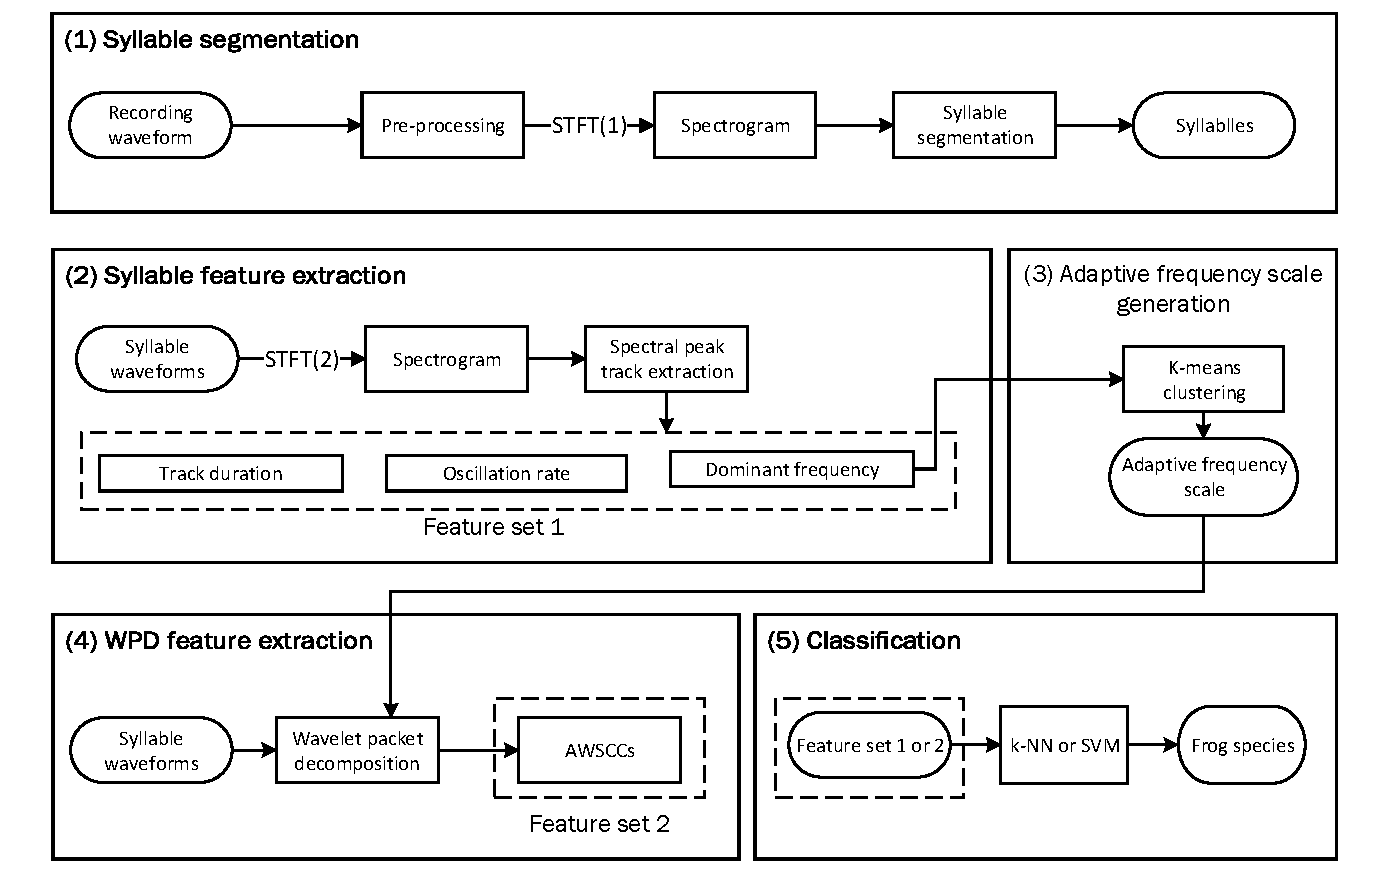
\includegraphics[width=1\linewidth]{image/Ch5/flowchart.pdf}}
\caption[Block diagram of the frog call classification system for wavelet-based feature extraction]{Block diagram of the frog call classification system. The line of dashes indicates the extracted feature set. AWSCCs is the abbreviation of \textit{adaptive wavelet packet decomposition sub-band cepstral coefficients}. STFT is short-time Fourier transform. For STFT(1), the window function, size and overlap are Kaiser window, 512 samples and 25\%. For STFT(2), the window function, size and overlap are Hamming window, 128 samples and 90\%. In this diagram, two feature sets are extracted, the description of other feature sets is shown in Figure~\ref{fig:featureExtraction}.}
\label{fig:Ch5_flowchart} 
\end{figure}


\subsection{Sound recording and pre-processing}

Two datasets obtained from a commercial recording \citep{CD} and James Cook University (JCU) were selected for this chapter. 
Recordings, which were collected from the CD, are two-channel, sampled at 44.10 kHz and saved in MP3 format. All recordings were obtained with a directional microphone and have a high signal to noise ratio (SNR). Each recording includes one frog species, and has a duration ranging from twenty-one to fifty-four seconds. The calls of eighteen frog species recorded in Queensland, Australia were used to develop the detailed methodology described in Figure~\ref{fig:Ch5_flowchart}. To reduce the subsequent computational burden, all the recordings selected from the CD were re-sampled at 16 kHz per second, mixed to mono, and saved in WAV format. 

The JCU recordings were obtained from Kiyomi dam (S $19^{\circ}$ $22^{'}$ $16.0^{''}$, E $146^{\circ}$ $27^{'}$ $31.3^{''}$)  BG Creek dam (S $19^{\circ}$ $27^{'}$ $1.23^{''}$, E $146^{\circ}$ $24^{'}$ $5.65^{''}$ ) and Stony Creek dam (S $19^{\circ}$ $24^{'}$ $07.0^{''}$, E $146^{\circ}$ $25’$ $51.3”$) in Townsville, using Song Meter (SM2) \citep{songMeter}. The recordings were stored on 16 GB SD cards in 64 kbps MP3 mono format and have a low SNR compared with the commercial recording. The sample rate is 16.00 kHz.
All the JCU recordings started around sunset, finished around sunrise every day and have 12 hour duration. 




%All the recordings in this study were collected from David Stewart's CD \citep{CD}. Recordings are two-channel, sampled at 44.10 kHz and saved in MP3 format. Each recording includes one frog species, with the duration ranging from twenty-one to fifty-four seconds. Eighteen frog species calls recorded in Queensland, Australia were used to develop the detailed methodology.   
%To reduce the subsequent calculation burden, all recordings were re-sampled at 16 kHz per second, mixed to mono, and saved in WAV format.


\subsection{Spectrogram analysis for validation set}
In this chapter, three syllables for each frog species are set aside and used as a \textit{reference data set}. For the commercial recording, three parameters including syllable duration, dominant frequency, and oscillation rate, are manually calculated for those three syllables of each species and averaged, as listed in Table \ref{tab:parameter}. The reference data set is excluded from the data used in the testing stage. 

\begin{table}[htb!]
\centering
\caption[Parameters of 18 frog species averaged of three
randomly selected syllable samples in the commercial recording]{Parameters of 18 frog species averaged of three
randomly selected syllable samples in the commercial recording. These selected samples make the \textit{reference data set}.}
\label{tab:parameter}
\resizebox{0.85\textwidth}{!}{
\begin{tabular}{llllll}
\hline\hline
{\bf No.} & {\bf Scientific name}         & {\bf Abbreviation} & {\bf \begin{tabular}[c]{@{}l@{}}Syllable duration\\  (millisecond)\end{tabular}} & {\bf \begin{tabular}[c]{@{}l@{}}Peak \\ frequency (Hz)\end{tabular}} & {\bf \begin{tabular}[c]{@{}l@{}}Oscillation rate \\ (cycle/second)\end{tabular}} \\ \hline
1         & Assa darlingtoni              & ADI                & 80                                                                               & 3200                                                                 & 160                                                                              \\ 
2         & Crinia parinsignifera         & CPA                & 250                                                                              & 4300                                                                 & 350                                                                              \\ 
%2         & Crinia signifera*              & CSA                & 90                                                                               & 2600                                                                 & 25                                                                               \\ \hline
%3         & Limnodynastes tasmaniensis*    & LAS                & 300                                                                              & 1600                                                                 & 20                                                                               \\ \hline
%5         & Limnodynastes terraereginae   & LTE                & 40                                                                               & 1000                                                                 & 1000                                                                             \\ \hline
3         & Litoria caerulea              & LCA                & 500                                                                              & 500                                                                  & 50                                                                               \\ 
4         & Litoria chloris               & LCS                & 800                                                                              & 1700                                                                 & 220                                                                              \\ 
5         & Litoria fallax                & LFX                & 430                                                                              & 4700                                                                 & 70                                                                               \\ 
6         & Litoria gracilenta            & LGA                & 1400                                                                             & 2700                                                                 & 100                                                                              \\ 
7        & Litoria latopalmata           & LLA                & 30                                                                               & 1400                                                                 & 2100                                                                             \\ 
8        & Litoria nasuta                & LNA                & 100                                                                              & 2800                                                                 & 160                                                                              \\ 
9        & Litoria revelata              & LRA                & 160                                                                              & 4100                                                                 & 70                                                                               \\ 
10        & Litoria rubella               & LUA                & 500                                                                              & 2900                                                                 & 60                                                                               \\ 
%10        & Litoria tyleri*                & LTI                & 700                                                                              & 2500                                                                 & 8                                                                                \\ \hline
11        & Litoria verreauxii verreauxii & LVV                & 270                                                                              & 3100                                                                 & 125                                                                              \\ 
12        & Mixophyes fasciolatus         & MFS                & 200                                                                              & 1200                                                                 & 140                                                                              \\ 
13        & Mixophyes fleayi              & MFI                & 50                                                                               & 1000                                                                 & 140                                                                              \\ 
%14        & Neobatrachus sudelli*          & NSI                & 480                                                                              & 1200                                                                 & 20                                                                               \\ \hline
14        & Philoria kundagungan          & PKN                & 170                                                                              & 430                                                                  & 95                                                                               \\ 
15        & Pseudophryne coriacea         & PCA                & 300                                                                              & 2400                                                                 & 80                                                                               \\
16        & Pseudophryne raveni           & PRI                & 370                                                                              & 2500                                                                 & 45                                                                               \\ 
17        & Rheobatrachus silus           & RSS                & 510                                                                              & 1500                                                                 & 60                                                                               \\ 
%19        & Uperoleia fusca              & UFA                & 550                                                                              & 2300                                                                 & 45                                                                               \\ \hline
18        & Uperoleia laevigata           & ULA                & 450                                                                              & 2400                                                                 & 150                                                                              \\ \hline\hline
\end{tabular}
}
\end{table}


For the JCU recordings\footnote[2]{https://www.ecosounds.org/}, the corresponding parameters are described in Table \ref{tab:JCU}. Compared with the commercial recordings from the CD, peak frequency shows a smaller variation than syllable duration and oscillation rate.


\begin{table}[htb!]
\centering
\caption[Parameters of eight frog species obtained by averaging three
randomly selected syllable samples from recordings of James Cook University]{Parameters of eight frog species obtained by averaging three
randomly selected syllable samples from recordings of James Cook University. NA indicates there is no oscillation structure in the spectrogram for the background noise and frog chorus. Since syllable durations of \textit{Rhinella marina} (Commom name: Canetoad) are very different from each other, we manually set the duration of Canetoad using the maximum duration of other frog species, which is 500 milliseconds.}
\label{tab:JCU}
\resizebox{0.85\textwidth}{!}{
\begin{tabular}{llllll}
\hline\hline
\textbf{No.} & \textbf{Scientific name}    & \textbf{Abbreviation} & \textbf{\begin{tabular}[c]{@{}l@{}}Syllable duration\\  (millisecond)\end{tabular}} & \textbf{\begin{tabular}[c]{@{}l@{}}Peak\\ frequency (Hz)\end{tabular}} & \textbf{\begin{tabular}[c]{@{}l@{}}Oscillation rate \\ (cycles/second)\end{tabular}} \\ \hline
1            & Rhinella marina                    & CTD                   & 500                                                                                 & 680                                                                    & 12                                                                                   \\ 
2            & Cyclorana novaehollandiae   & CNE                   & 350                                                                                 & 600                                                                    & NA                                                                                   \\ 
3            & Limnodynastes terraereginae & LTE                   & 80                                                                                  & 630                                                                    & NA                                                                                   \\ 
4            & Litoria fallax              & LFX                   & 120                                                                                 & 4100                                                                   & 50                                                                                   \\ 
5            & Litoria nasuta              & LNA                   & 100                                                                                 & 2700                                                                   & NA                                                                                   \\ 
6            & Litoria rothii              & LRI                   & 350                                                                                 & 1150                                                                   & 15                                                                                   \\ 
7            & Litoria rubella             & LUA                   & 500                                                                                 & 2400                                                                   & NA                                                                                   \\ 
8            & Uperolela mimula            & UMA                   & 120                                                                                 & 2400                                                                   & 40                                                                                   \\ \hline\hline
\end{tabular}
}
\end{table}




\subsection{Syllable segmentation}



%For frog calls, an elementary acoustic unit for classification is the syllable, which is a continuous vocalisation emitted from an individual \citep{huang2009frog}. Each commercial recording consists of multiple continuous calls of one frog species. Therefore, it is necessary to segment each call into individual syllables. This syllable segmentation process is applied to the spectrogram, which is generated by applying short-time Fourier transform (STFT) to each recording. For STFT, the window function is the Hamming window with the size and overlap of 512 samples and 25\%, respectively. 

The syllable segmentation process is described in Chapter \ref{Ch3:segmentationProcess}. To further improve the segmentation result, the averaged energy of which is less than 15\% of the maximum energy, are removed \citep{Gingras2013}. The distribution of syllable numbers after segmentation for all frog species is shown in Figure~\ref{fig:Ch5_syllable}.

%For recordings from James cook university, syllable segmentation is not necessary, because 30 syllables of each frog species are manually selected.

For the JCU recordings, bandpass filtering is applied to each recording before using the H$\ddot{a}$rm$\ddot{a}$'s method \citep{harma2003automatic}. A bandpass filter is first used to filter specific frog species, because different frog species tend to call simultaneously.   The filtering is 

$$ S^{'}(t,f) =\left\{
\begin{array}{rcl}
 S(t,f) && F_{lower} \leq f \leq F_{upper}  \\
0 \\
\end{array}
\right.
$$
Here, $S^{'}(t,f)$ is the filtered spectrogram, the $F_{lower}$ and  $F_{upper}$ are lower and upper cutoff frequency and calculated as 
\begin{equation}
\begin{aligned}
F_{upper} = F_{peak} + \beta \\
F_{lower} = F_{peak} - \beta
\end{aligned}
\end{equation}
\noindent where $F_{peak}$ is the peak frequency (Table \ref{tab:JCU}), $\beta$ is a threshold for determining the frequency bandwidth and set at 300 Hz based on the \textit{reference data set}.

After bandpass filtering, noise reduction is essential for
improving the segmentation result for the low
signal to noise ratio in JCU recordings. Here, we use the method of \cite{towsey2012toolbox} for noise reduction. Finally, we use the H$\ddot{a}$rm$\ddot{a}$'s method to detect individual syllables (Figure~\ref{fig:Ch5_segmentation}). 



For the JCU recordings, eight frog species were used for the experiment. After syllable segmentation of continuous recordings, for each frog species, we randomly selected 30 syllables from segmentation results for subsequent analysis.


\begin{figure}[htb!] % Example image
\center{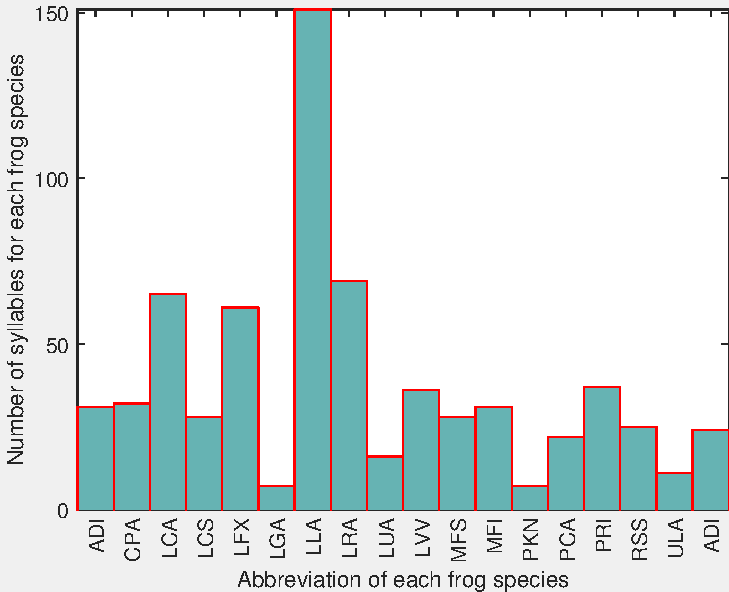
\includegraphics[width=0.6\linewidth]{image/Ch5/syllable.pdf}}
\caption[Distribution of number of syllables for all frog species]{Distribution of syllable number for all frog species. The x-axis is the abbreviation of each frog species, and the corresponding scientific name can be found in Table \ref{tab:parameter}.}
\label{fig:Ch5_syllable} 
\end{figure}





\begin{figure}[htb!]
\centering
        \begin{subfigure}[b]{0.5\textwidth}
                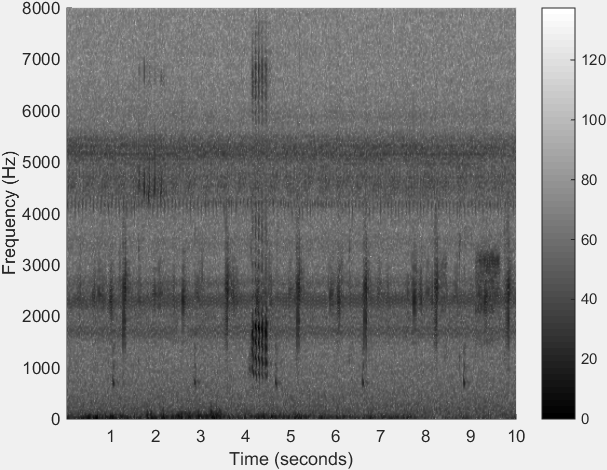
\includegraphics[width=\textwidth]{image/Ch5/spectrogram.png}
                \caption{Spectrogram.}
        \end{subfigure}%
        \\ 
        \begin{subfigure}[b]{0.5\textwidth}
                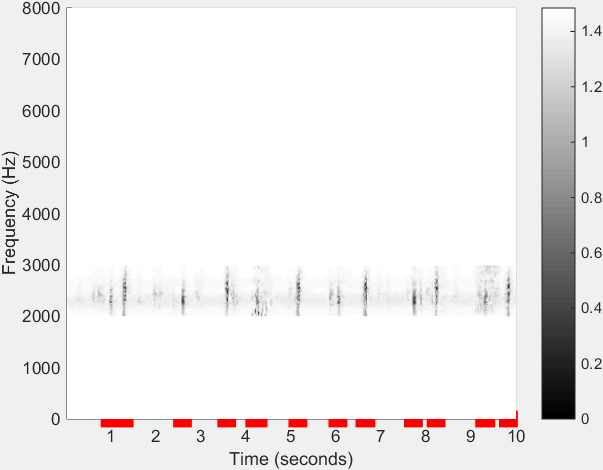
\includegraphics[width=\textwidth]{image/Ch5/segmentation.png}
                \caption{Segmentation results with marked red lines.}
        \end{subfigure}
%        \\
%                \begin{subfigure}[b]{0.23\textwidth}
%                \includegraphics[width=\textwidth]{image/noiseReduction.png}
%                \caption{Noise reduction}
%        \end{subfigure}%
%        ~ 
%        \begin{subfigure}[b]{0.23\textwidth}
%                \includegraphics[width=\textwidth]{image/segmentationResult.png}
%                \caption{Segmentation results}
%        \end{subfigure}
        \caption[Segmentation results based on bandpass filtering]{Segmentation results  for \textit{Uperolela mimula} using bandpass filtering, noise reduction and H$\ddot{a}$rm$\ddot{a}$'s method. The red line in (b) indicates the start and stop location of each segmented syllable.}       
        \label{fig:Ch5_segmentation}
\end{figure}



%\begin{figure}[htb!] % Example image
%\center{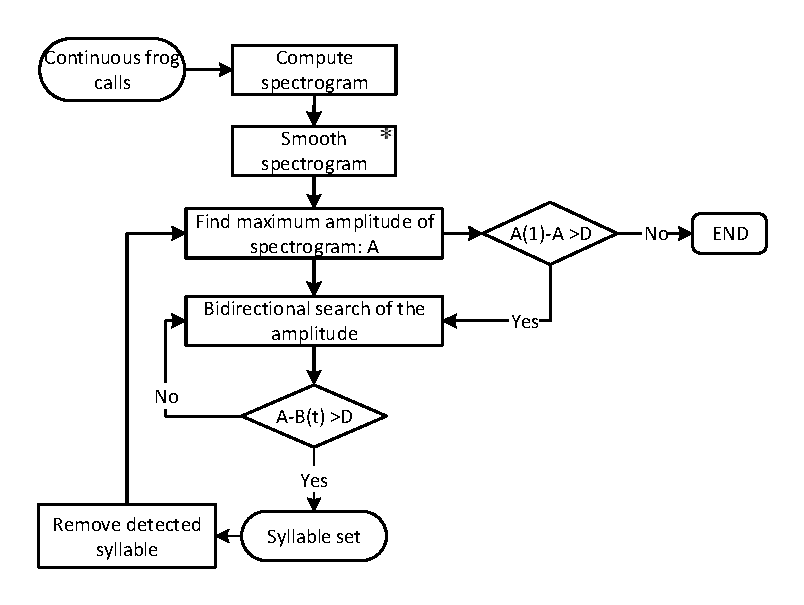
\includegraphics[width=1\linewidth]{image/segmentation.pdf}}
%\caption{Segmentation method based on H$\ddot{a}$rm$\ddot{a}$'s algorithm. Here, $D$ is the amplitude threshold for stopping criteria which is set at 20 dB experimentally, and the segmentation result is sensitive with this value. $A$ is the maximum amplitude value of the spectrogram and we save the first maximum amplitude as $A(1)$, $B(t)$ is the amplitude of frame $t$. An asterisk denotes the optional processing step.}
%\label{fig:segmentation} 
%\end{figure}



%In this study, smoothing spectrogram is optionally applied to the spectrogram before H$\ddot{a}$rm$\ddot{a}$'s algorithm, because some frog species have large temporal gap within one syllable (see in Figure~\ref{fig:smooth}). Here, oscillation rate of the validation set is to used to decide which frog species need to be smoothed. Oscillation rate ($O_{r}$) represents the number of pulses within one second. The algorithm for extracting oscillation rate is introduced in our previous work \citep{Xie1504:Acoustic}, which is summarized as follows. Different from the previous work, the frequency boundary for calculating power vector is based on the peak frequency in Table.\ref{tab:parameter} rather than the dominant frequency, because the dominant frequency has not been calculated. Here, the low and high frequency boundary is 500 Hz and 4500 Hz.  After defining the frequency band, the power vector is calculated and normalized, and the first and last 20\% part of the vector is discarded, because of the unclear of the start and end of the syllables. Next, the autocorrelation with the length of the vector is calculated. Furthermore, a discrete cosine transform (DCT) is applied to the vector after subtracting the mean, and the position of the highest frequency ($P_{f}$) is achieved. Finally, the oscillation rate is defined as
%\begin{equation}
%O_{r}= \frac{P_{f}}{L_{dct}}*r_{x}*\gamma
%\end{equation}
%\noindent where $P_{f}$ is the position of the highest frequency values of the DCT result, $L_{dct}$ is the length for applying DCT to the power vector, and is experientially set as 0.2 second in this study. The results of the oscillation rate is shown in Figure~\ref{fig:osc}.  In the testing stage, the oscillation rate of one randomly selected syllables from continuous audio data is calculated, then compared to decide whether to smooth or not. When the oscillation rate is lower than 40 cycles/second, a Gaussian filter (7$\times$7) is applied to the spectrogram. Here, the filter size is set taking into account a trade-off between connecting gaps within one syllable and separating adjacent syllables.
%The segmentation result after smoothing is shown in Figure~\ref{fig:smooth}.
%
%\begin{figure}[htb!] % Example image
%\center{\includegraphics[width=0.65\linewidth]{image/thresh.pdf}}
%\caption{Oscillation rate of the validation set for 20 frog species. The horizontal line represents the threshold for smoothing, which is set as 40 cycles/second experimentally.}
%\label{fig:osc} 
%\end{figure}
%
%
%
%\begin{figure}[htb!]
%\centering
%        \begin{subfigure}[b]{0.6\linewidth}
%                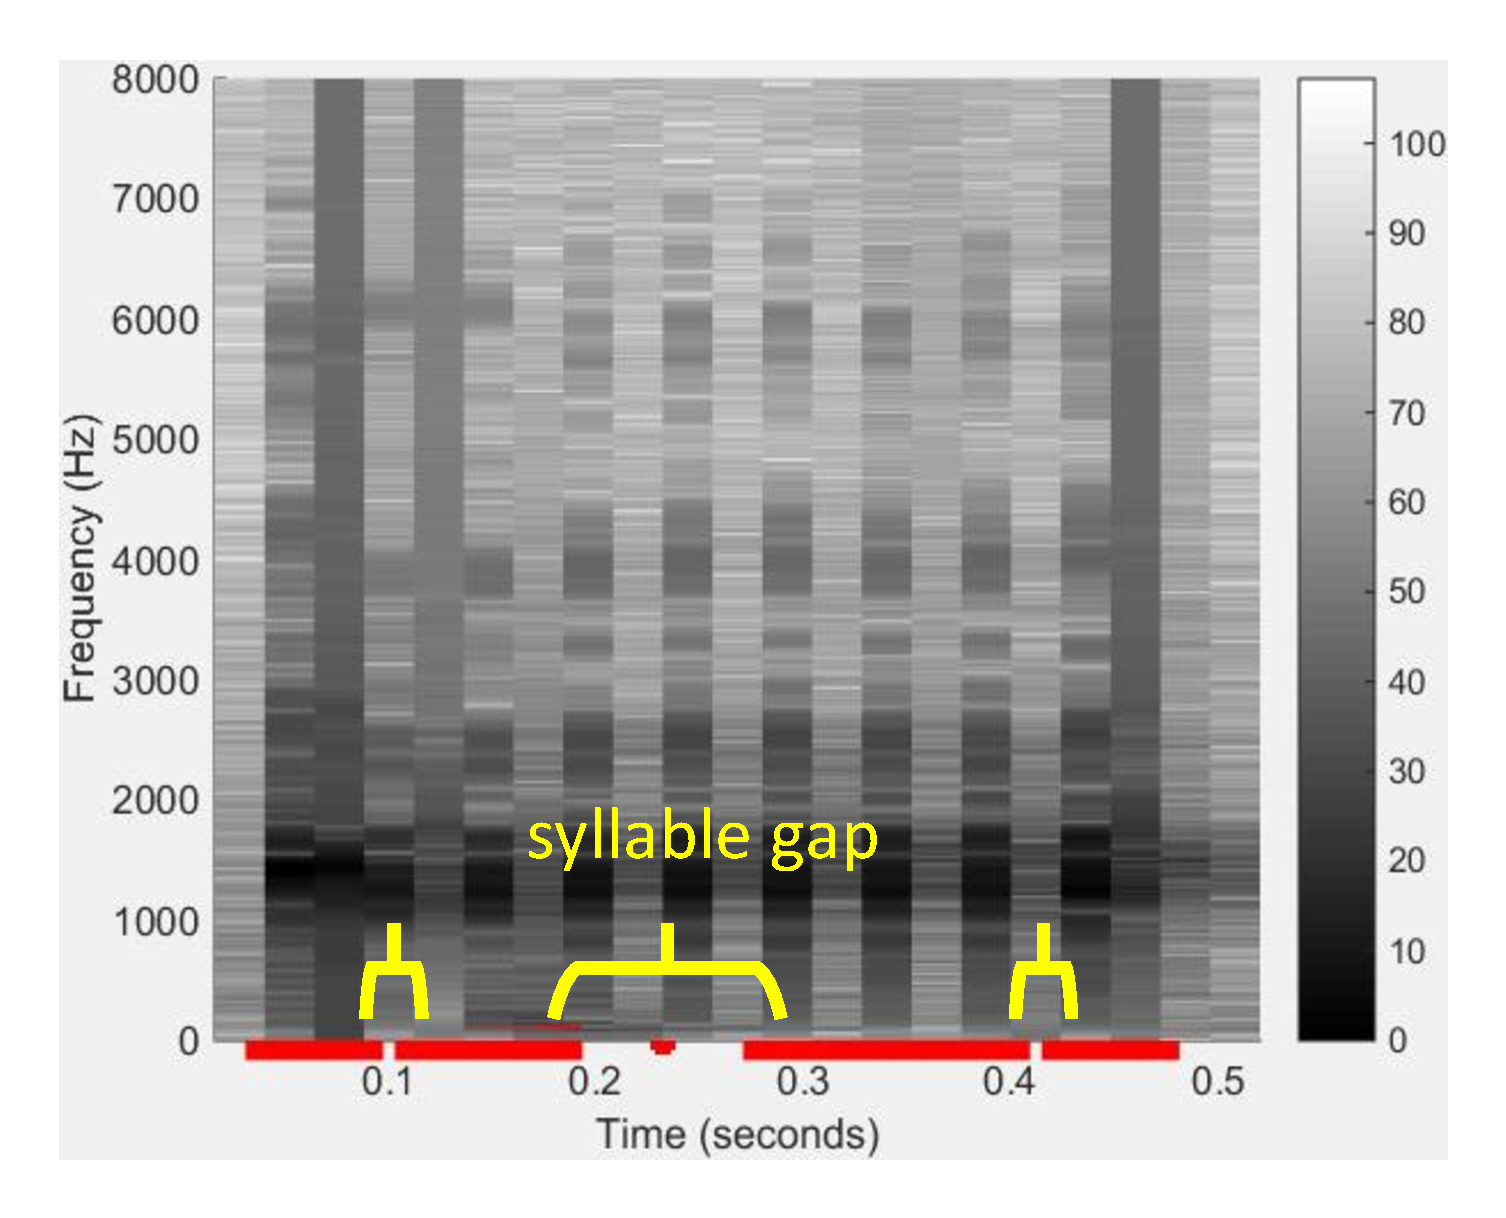
\includegraphics[width=\textwidth]{image/no.pdf}
%                \caption{Before smoothing}
%        \end{subfigure}%
%        \\ 
%        %add desired spacing between images, e. g. ~, \quad, \qquad, \hfill etc.
%          %(or a blank line to force the subfigure onto a new line)
%        \begin{subfigure}[b]{0.6\linewidth}
%                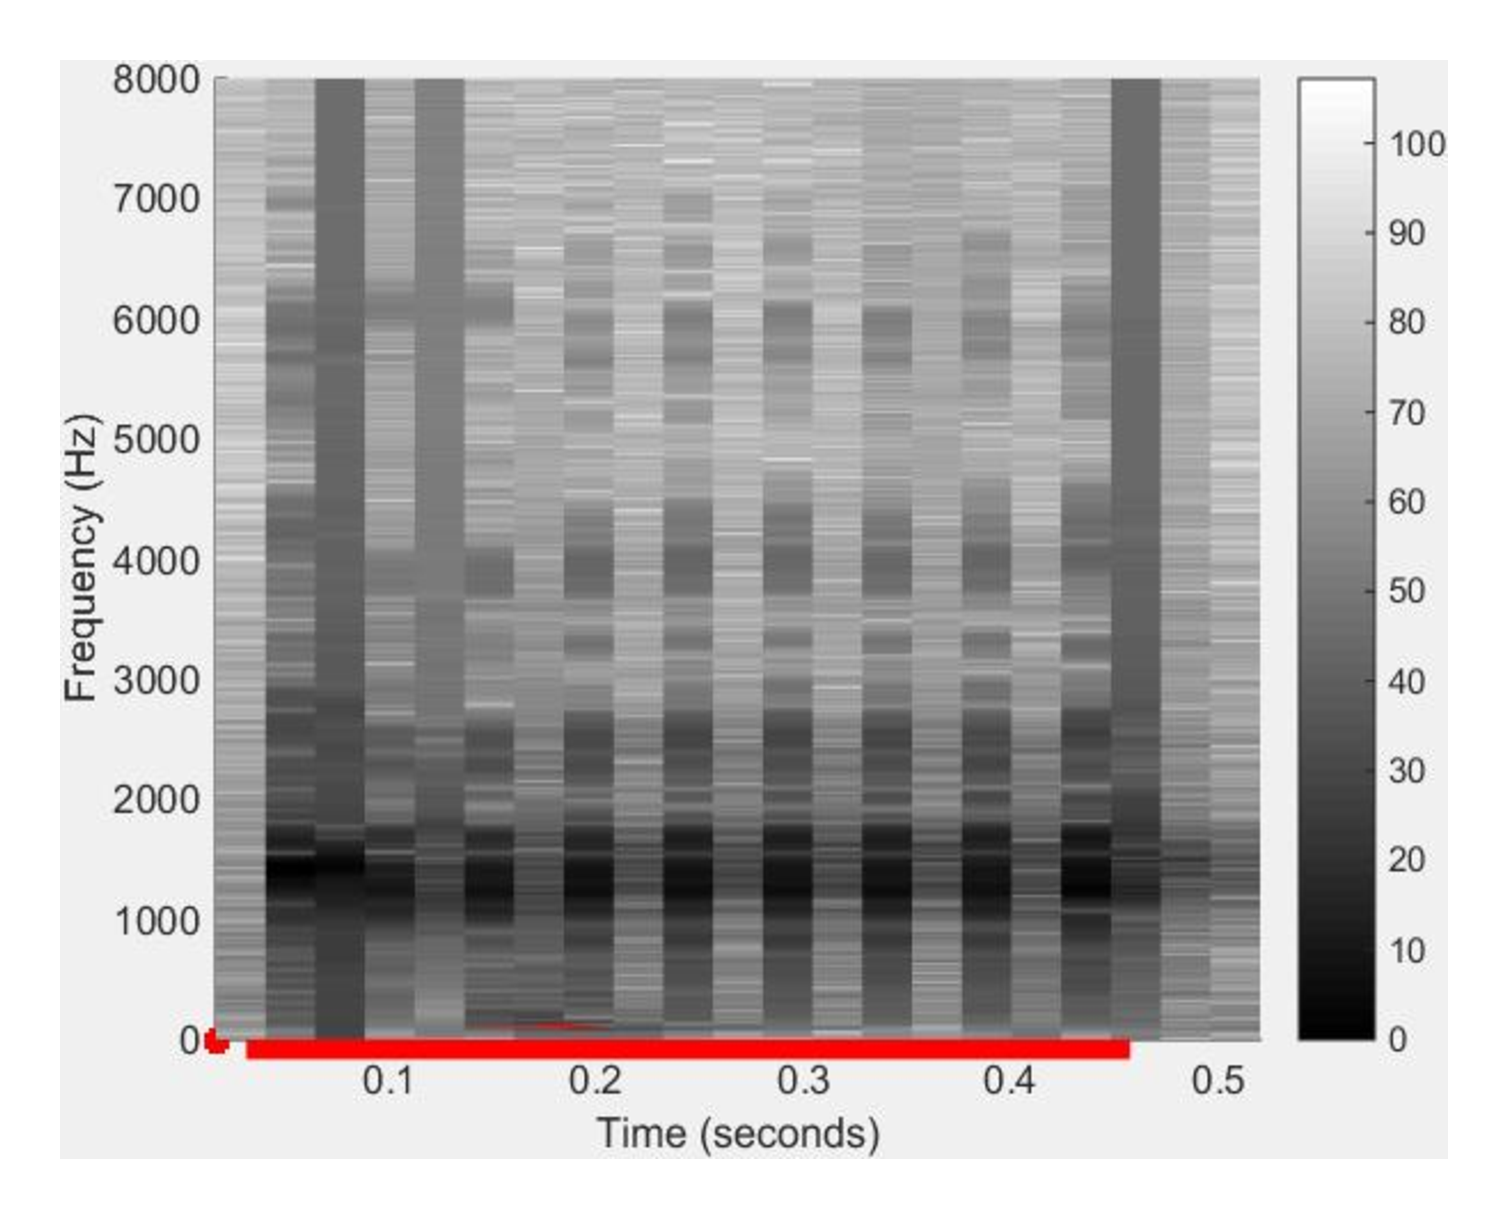
\includegraphics[width=\textwidth]{image/yes.pdf}
%                \caption{After smoothing}
%        \end{subfigure}
%        \caption{Syllable segmentation results are marked with red
%line for \textit{Neobatrachus sudelli} (one syllable).}       
%        \label{fig:smooth}
%\end{figure}
 


\subsection{Spectral peak track extraction}
Spectral peak tracks (SPT) (also called frequency tracks) have been explored for studying birds \citep{birdTrack, jasaTrack} and whales \citep{roch2011automated}. In this chapter, the spectral peak track is used to represent the trace of a frog advertisement call, because frogs that are genetically related share more similar advertisement calls than distantly related frogs \citep{Gingras2013}. The reasons for using SPT are (1) to isolate the desired frog calls from the background noise; (2) to extract corresponding SPT features. Here, the SPT method is reported in \citep{Xie1504:Acoustic}. 

For the SPT extraction algorithm, seven parameters need to be set (Table \ref{tab:SPT}). The process for determining those parameters is explained in Section 3. 

\begin{table}[htb!]
\centering
\caption{Parameters used for spectral peak extraction}
\label{tab:SPT}
\resizebox{0.85\textwidth}{!}{
\begin{tabular}{ll}
\hline\hline
{\bf Parameter} & {\bf Description}                                     \\ \hline
   $I$ (dB)             & Minimum intensity threshold for peak selection        \\ 
   $T_{c}$ (s)             & Maximum time domain interval for peak connection      \\ 
     $T_{s}$ (s)           & Minimum time interval for stopping growing tracks     \\ 
     $f_{c}$ (Hz)          & Maximum frequency domain interval for peak connection \\ 
     $d_{min}$ (s)           & Minimum track duration                                \\ 
    $d_{max}$ (s)            & Maximum track duration                                \\ 
    $\beta$ (0$\sim$1)            & Minimum density value                                 \\ \hline\hline
\end{tabular}
}
\end{table}

Before applying the SPT extraction algorithm, each syllable is transformed to a spectrogram with the following parameter settings (Hamming window, frame size is 128 samples, and window overlap is 90\%). For the generated spectrogram, the maximum intensity (real peak) is selected from each frame with a minimum required intensity, $I$. Then, the time and frequency domain intervals between two successive peaks are calculated. If the time and frequency intervals are smaller than $T_{c}$ and $f_{c}$ respectively, one initial track (SPT$_{1}$) will be generated. After that, linear regression is applied to the generated track for calculating the position of the next predicted peak. Based on peaks $p_{1}(t_{1},f_{1})$ and $p_{2}(t_{2},f_{2})$ within the initial track (SPT$_{1}$), $a$ and $b$ in Equation (4.2) can be solved. 

\begin{equation}
f= at+b
\end{equation}

Based on $a$ and $b$, the predicted peak $\hat{p_{n}}$ of the following frame $t_{n}$ can be calculated. 
Next, the time and frequency domain intervals between predicted peak ($\hat{p_{n}}$) and the real peak of the successive frame are recalculated. If the time and frequency intervals are smaller than $T_{c}$ and $f_{c}$ respectively, the real peak will be added to the initial track. After each peak is added to the initial track, linear regression is repeated to recalculate the next predicted peak using at most the last 10 included peaks. This iterative process continues until $T_{s}$ is no longer satisfied. 
When no more peaks will be added to one track, the next step is to compare the duration and density of the track with $d_{min}$, $d_{max}$, and $\beta$. If all conditions are satisfied, then the track will be saved to the track list. The SPT results for \textit{Neobatrachus sudelli} are shown in
Figure~\ref{fig:track}. During the process of track extraction, time domain gaps  are generated where the intensity threshold $I$ is not reached.
These gaps can be filled by predicting the correct frequency
bin using linear regression, as illustrated in Figure~\ref{fig:track}. 

\begin{figure}[htb!]
\centering
        \begin{subfigure}[b]{0.5\textwidth}
                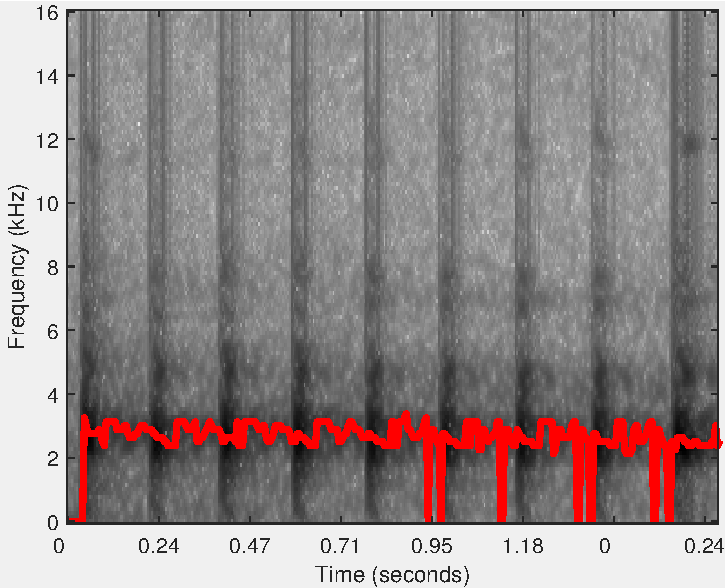
\includegraphics[width=\textwidth]{image/Ch5/peak.pdf}
                \caption{selected peaks below the intensity threshold $I$ are set to zero.}
        \end{subfigure}%
        \\ 
        %add desired spacing between images, e. g. ~, \quad, \qquad, \hfill etc.
          %(or a blank line to force the subfigure onto a new line)
        \begin{subfigure}[b]{0.5\textwidth}
                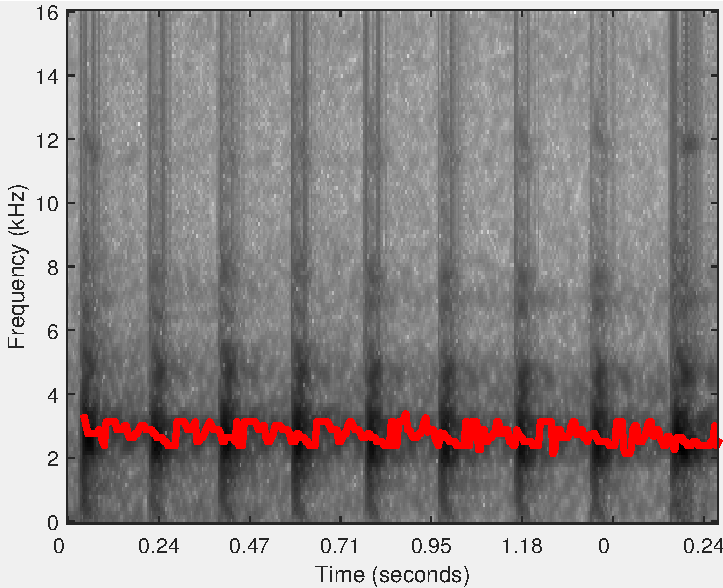
\includegraphics[width=\textwidth]{image/Ch5/track.pdf}
                \caption{spectral peak track with predicted peaks using linear regression.}
        \end{subfigure}
        \caption[Spectral peak track extraction results]{Spectral peak track extraction results for \textit{Neobatrachus sudelli}. By filling the gaps within the track, the dominant frequency can be more accurately calculated.}       
        \label{fig:track}
\end{figure}

\subsection{Syllable SPT features}

After SPT extraction, each SPT is expressed in the following format: (1) track start time $t_{s}$; (2) track stop time $t_{e}$; (3) frequency bin index for each of the peaks within the track $f_{t}$ ($t_{s} \leq t \leq t_{e}$).  Then, syllable features including track duration, dominant frequency, and oscillation rate are calculated based on the SPT.

\noindent \textbf{a)} Track duration (second):
Track duration ($D_{t}$) is directly obtained from the bounds of the track.
\begin{equation}
D_{t} = (t_{e}-t_{s})*r_{x}
\end{equation}
\noindent where $r_{x}$ is the time domain resolution in unit second per frame.

\noindent \textbf{b)} Dominant frequency (Hz): 
Dominant frequency ($\bar{f}$) is calculated by averaging the frequency of all peaks within one track
\begin{equation}
\bar{f} = \sum_{t=t_{s}}^{t_{e}}f_{t}/(t_{e}-t_{s}+1)*r_{y}
\end{equation}
where $r_{y}$ is the frequency domain resolution with unit frequency per bin, $f_{t}$ is the frequency bin index of peak $t$.

\noindent  \textbf{c)} Oscillation rate (Hz):  
Oscillation rate ($O_{r}$) represents the number of pulses per second. The algorithm for extracting oscillation rate is introduced and summarised as follows.
First, the frequency domain boundary is defined based on the dominant frequency, and the power within the boundary is calculated. Then, the power vector is normalised, and the first and last 20\% part of the vector is discarded, because of the uncertainty in the start and end of the syllables. Next, the autocorrelation with the length of the vector is calculated. Furthermore, a discrete cosine transform (DCT) is applied to the vector after subtracting the mean, and the position of the highest frequency ($P_{f}$) is achieved. Finally, the oscillation rate is defined as
\begin{equation}
O_{r}= \frac{P_{f}}{L_{dct}}*r_{x}*\gamma
\end{equation}
\noindent where $P_{f}$ is the position of the highest frequency values of the DCT result, $L_{dct}$ is the length for applying DCT to the power vector, and is experientially set as 0.2 second in this chapter. 



\subsection{Wavelet packet decomposition}
Wavelet packet decomposition (WPD) is a powerful tool for the analysis of non-stationary signals, which includes multiple bases and different basis \citep{selin2007wavelets}. With WPD, an original acoustic signal can be split into two frequency bands such as lower and higher frequency band. Then, both lower and higher frequency bands can be further continuously decomposed into two sub-bands, which produce a complete wavelet packet tree \citep{farooq2001mel}. Due to its ability for analysing a non-stationary signal, WPD has been used to analyse acoustic signals \citep{selin2007wavelets, ren2008perceptually}. Here, WPD is used to obtain features for frog call classification. 

\subsection{WPD based on an adaptive frequency scale}
To obtain robust features for frog call classification, the frequency scale used for WPD is crucial. In prior work \citep{barkWPDraey, Biswas20141111, Zhang2015108}, different frequency scales have already been proposed for WPD. Bark-scaled WPD was proposed by Litvin and Cohen to separate blind source from a single channel audio source \citep{barkWPDraey}. \cite{Biswas20141111} used features based on ERB-scaled (Equivalent rectangular bandwidth) WPD for Hindi consonant recognition.  \cite{Zhang2015108} developed a method based on Mel-scaled WPD for bird sound detection with the SVMs classifier. However, most frequency scales used for WPD are developed for studying speech rather than frogs. Therefore, finding a suitable frequency scale for frogs to perform the WPD is important for obtaining features with strong discriminatory power. In this chapter, an adaptive frequency scale for WPD for frog calls is proposed,  based on the dominant frequency of frog species to be classified. Specifically, the k-means clustering algorithm is used to cluster the dominant frequency of all syllables. Then, the centroids of the clustering result are used to generate the frequency scale. Here, the value of $k$ for the k-means clustering algorithm is the same as the number of frog species to be classified, the distance function used is \textit{city block} \citep{Melter1987235}. 


%The k-means clustering result for the validation data set is shown in Figure~\ref{fig:kmeans}.
%
%
%\begin{figure}[htb!] % Example image
%\center{\includegraphics[width=0.65\linewidth]{image/k-means.pdf}}
%\caption{K-means clustering results for the dominant frequency of the validation set}
%\label{fig:kmeans} 
%\end{figure}




Based on the obtained frequency scale, an adaptive frequency scaled WPD method is proposed, which is described in Algorithm 1. The wavelet packet tree used for classifying 18 frog species is shown in Figure~\ref{fig:tree20}.


\begin{algorithm}
\DontPrintSemicolon
\KwData{ $c_{i}(i=1,2,...,K)$, $f_{s}$, where $K$ is the number of frog species to be classified, $c_{i}$ is the centroid of the clustering results, $f_{s} = sr / 2$ where $sr$ is the sample rate of the audio recordings, which is 16 kHz here.}
\KwResult{Adaptive wavelet packet tree}

\Begin{
%
\textbf{Step 1}: Sort the centroid $c_{i}(i=1,2,...,K)$, and calculate the difference between the consecutive vectors of $c$, sort the difference and save it as $d_{j}(j=1,2,...,K-1)$

\textbf{Step 2}: Calculate the decomposition level $L$ based on the following rule

$ f_{s}/min(d) \leq 2^{L-1}$

where L is the minimum integer that satisfies that equation. 

\textbf{Step 3}: Perform the wavelet packet decomposition

\For{$l =1:L$}{
\textbf{1}. Calculate the frequency resolution of level l

\For{$i = 1:K$}{

\textbf{1}: Put the $c_{i}$ into the right frequency band

\textbf{2}: Count the number of $c_{i}$ in each band ($n$)

}


\eIf{$ n \geq 2 $}{
perform further decomposition to that particular node
}{
stop decomposition
}
}

%\textbf{Step 4}:  further split each root node for improving the frequency resolution
}
\caption{Adaptive frequency scale for WPD}
\end{algorithm}



\begin{figure}[htb!] % Example image
\center{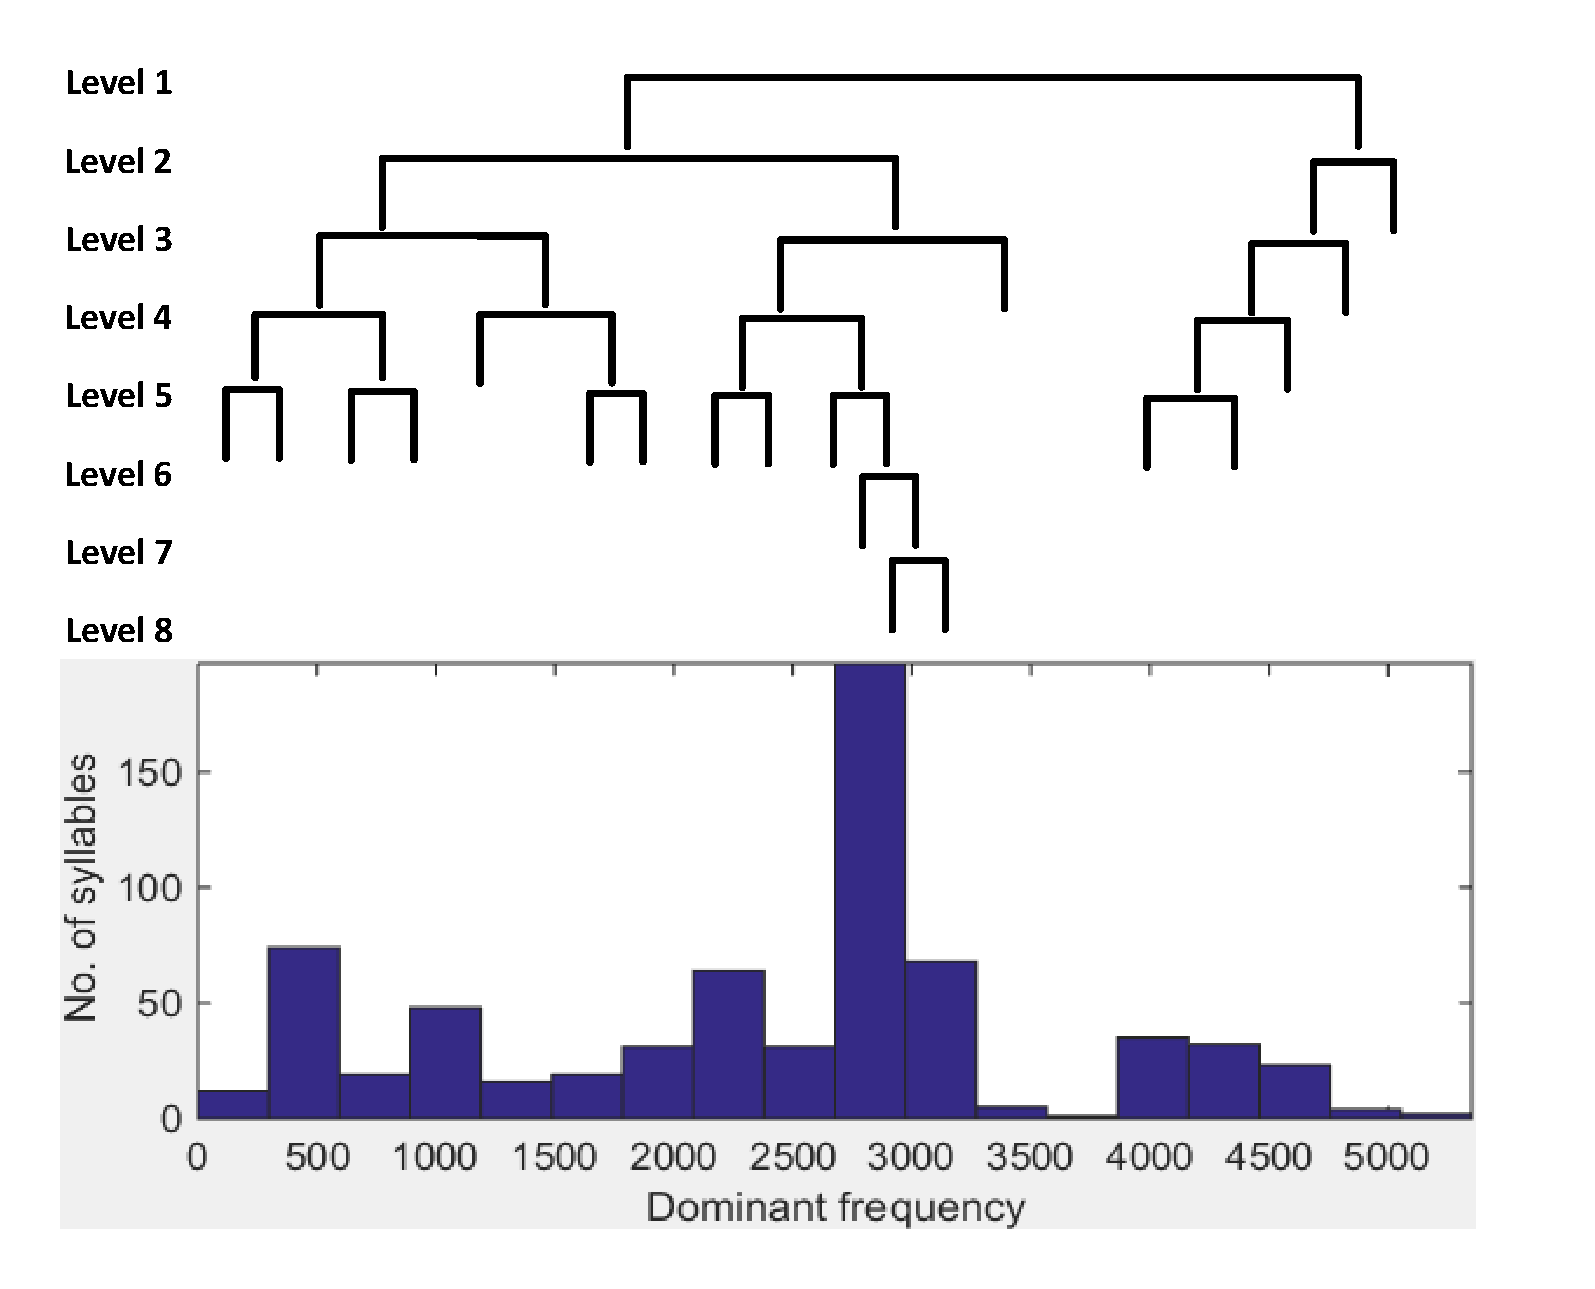
\includegraphics[width=0.65\linewidth, height = 0.65\linewidth]{image/Ch5/tree18.pdf}}
\caption[Adaptive wavelet packet tree for classifying twenty frog species]{Adaptive wavelet packet tree for classifying twenty frog species. The upper image is the wavelet packet tree; the lower image is the histogram of dominant frequency for twenty frog species.}
\label{fig:tree20} 
\end{figure}



\subsection{Feature extraction based on adaptive frequency scaled WPD}

%The aim of feature extraction is to obtain a sequence of feature vectors that hidden in the original time domain \citep{yen2000wavelet}.
In previous studies \citep{bedoya2014automatic, Xie1504:Acoustic}, Mel-frequency cepstral coefficients (MFCCs) have been used for studying bioacoustic data, and used as the baseline for feature comparison in this chapter. Besides MFCCs, another feature set called Mel-scaled wavelet packet decomposition sub-band cepstral coefficients (MWSCCs) is also included in the comparison experiment \citep{Zhang2015108}, because it shows better performance than MFCCs for bird detection in a complex environment. In this chapter, we propose a novel feature set named \textit{adaptive frequency scale wavelet packet decomposition sub-band cepstral coefficients} (AWSCCs) for frog call classification.
The extraction procedure of AWSCCs is similar to MWSCCs. However, the frequency scale used for our AWSCCs is based on an adaptive frequency scale rather than the Mel-scale for MWSCCs. Meanwhile, after performing DCT, temporal feature integration is used for calculating the statistics of feature vectors which generates different statistical types of AWSCCs. (see in Figure~\ref{fig:featureExtraction}). 


\begin{figure*}[htb!] % Example image
\center{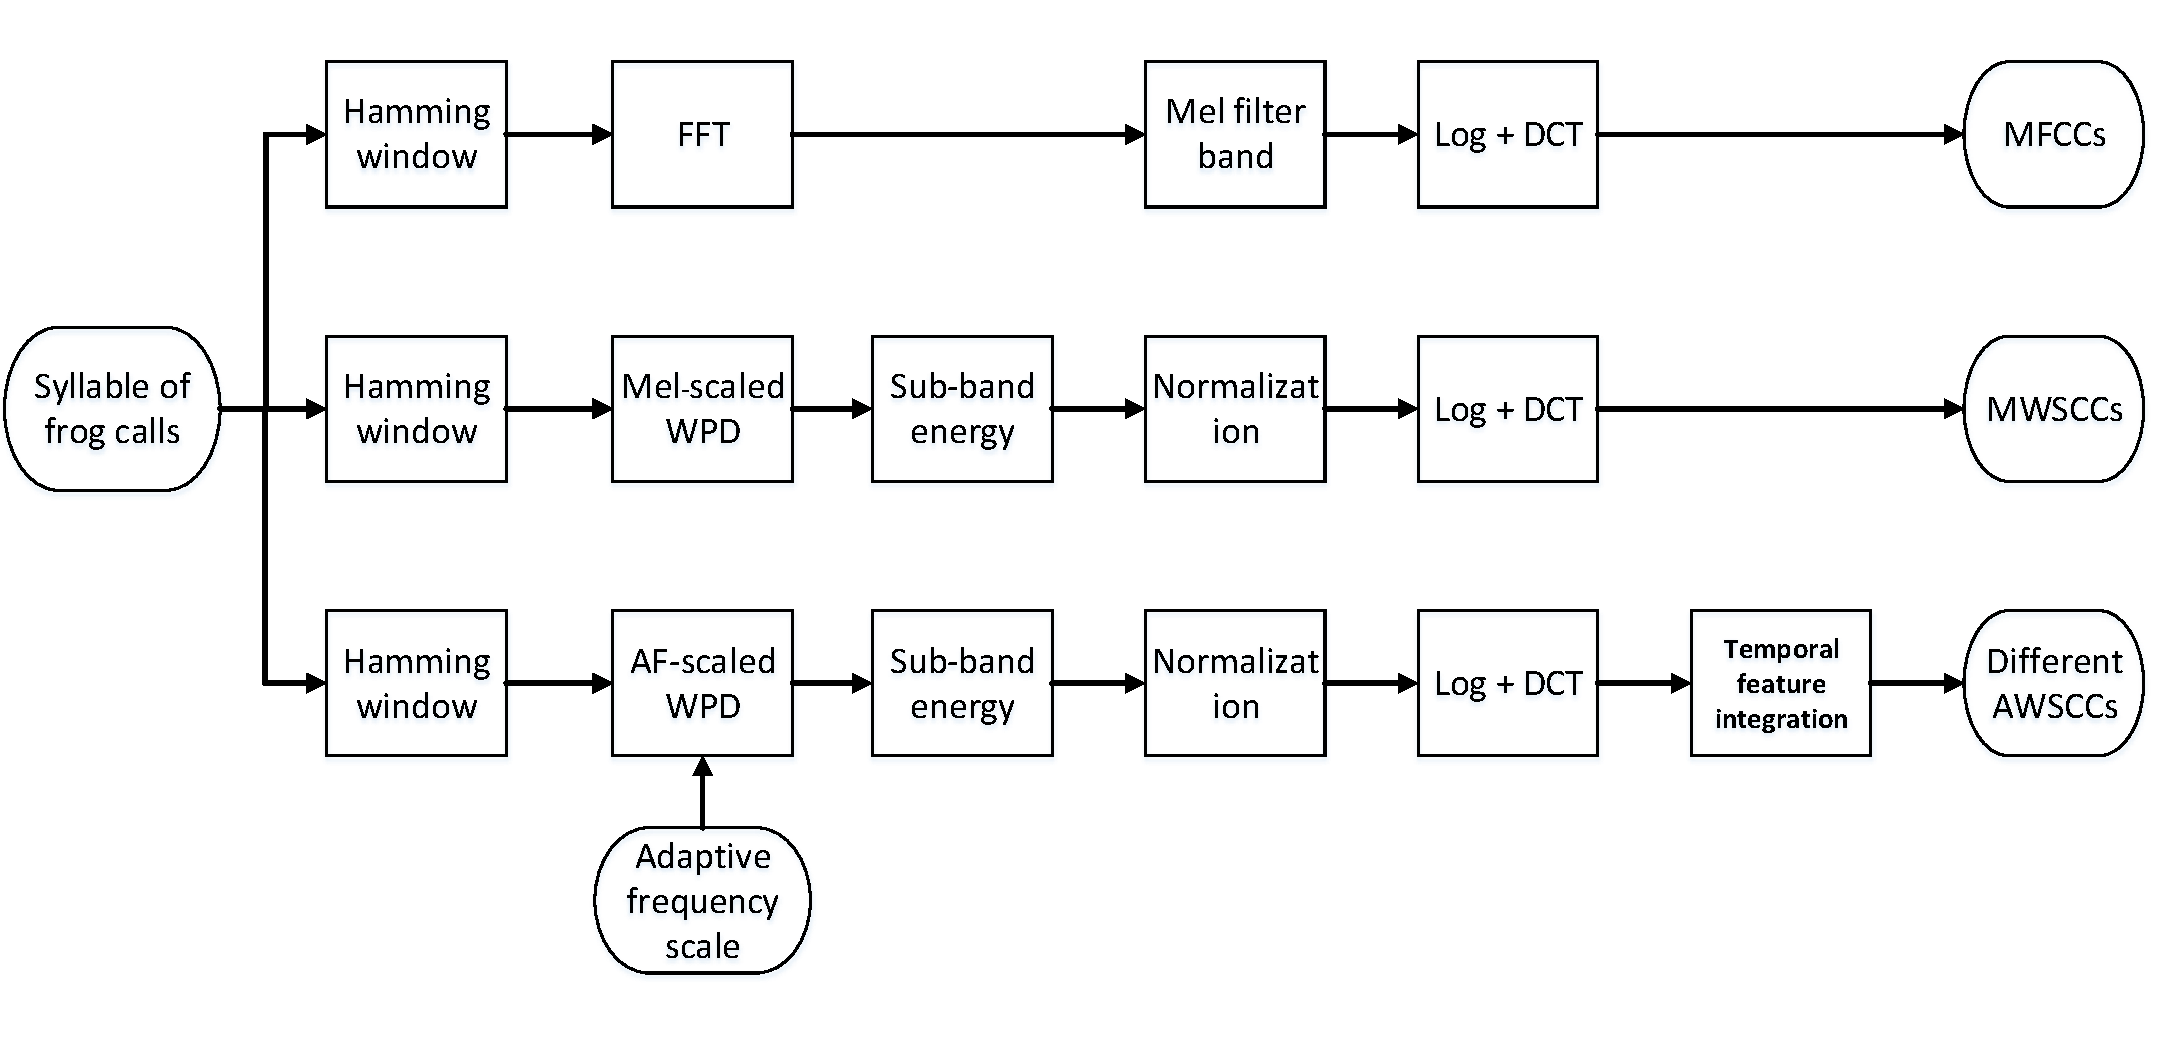
\includegraphics[width=1\linewidth, height=0.45\linewidth]{image/Ch5/featureExtraction.pdf}}
\caption{Description of three feature extraction methods including MFCCs, MWSCCs, and different statistical types of AWSCCs.}
\label{fig:featureExtraction} 
\end{figure*}


After syllable segmentation, the signal of one syllable is represented as 
$y(n),\,n = 1,...,N$, where $N$ is the length of one syllable of frog calls. Based on the $y(n)$, steps for AWSCCs extraction are described as follows:\\
\textbf{1)}. Add Hamming window to the signal $y(n)$.
\begin{equation}
x(n) = w(n)y(n)
\end{equation}
\noindent where $w(L)$ is the Hamming window function and defined as $w(n)=0.54-0.46cos(\frac{2n\pi}{L-1}) $, $L$ is the length of Hamming window and set as 128 samples here.
\\
\textbf{2)}. Perform wavelet packet decomposition spaced in adaptive frequency scale as described in Section 2.7.
\begin{equation}
WP(i,j)=\sum_{i=1}^{M}x(n)\psi_{(a,b)}(n) 
\end{equation}
\noindent where $WP(i,j)$ is the wavelet coefficients of the decomposition, $i$ is the sub-band index, $j$ is the index of wavelet coefficients, $\psi_{(a,b)}(n)$ is the wavelet base function, and we use 'Db 4' experimentally. Here, $a$ and $b$ are the scale and shift parameters, respectively. 'Db 4' represents the Daubechies wavelet transform which has four scaling and wavelet function coefficients.
\\
\textbf{3)}. Calculate the total energy of each sub-band.
\begin{equation}
WP_{i}=\sum_{j=1}^{M_{i}}[WP(i,j)]^2
\end{equation}
\noindent where $i=1,2,...,T$, and $T$ is the total number of sub-band, and $j=1,2,...,M_{i}$, $M_{i}$ is the total number of wavelet coefficients.
\\
\textbf{4)}. Normalise the energy of each sub-band.
\begin{equation}
SE_{i}=\frac{WP_{i}}{M_{i}}
\end{equation}
\noindent where $i=1,2,...,T$.
\\
\textbf{5)}. Perform DCT on the logarithm sub-band energy for dimension reduction and obtain the feature AWSCCs.
\begin{equation}
AWSCCs(d)=\sum_{i=1}^{T}logSE_{i}cos(\frac{d(i-0.5)}{T}\pi)
\end{equation}
\noindent where $d=1,2,...,d^{'}$, $1 \leq d^{'} \leq T$, here $d^{'}$ is the dimension of AWSCCs, and set as 12 here. To keep the feature dimension consistency, the dimensions for MFCCs and MWSCCs are also set as 12 in this chapter, and the detailed steps for extraction can be found in \citep{bedoya2014automatic} and \citep{Zhang2015108}.
\\
\textbf{6)}. Temporal feature integration
\\
Here, the statistics of all feature vectors over each windowed signal are calculated, which include sum, average, standard deviation, and skewness. With randomly selected five instances for each frog species, the classification accuracy of averaged AWSCCs is higher than other statistics of AWSCCs. Therefore, only averaged AWSCCs are used in the subsequent experiment. To capture the dynamic information of the frog calls, the delta-AWSCCs are also calculated based on the averaged AWSCCs. 




\subsection{Classification}
In this chapter, the k-nearest neighbour (k-NN) and support vector machine (SVM) classification algorithms are used for frog call classification. The input parameters for each classifier are syllable features (SFs), MFCCs, MWSCCs, and different AWSCCs, and the output is the frog species.
The descriptions of those two classifiers can be found in Chapter \ref{ch4:classifierDesign}.

%\subsubsection{k-nearest neighbours}
%For the k-NN classifier, an object is classified to the class of the majority of its k nearest neighbours \citep{huang2009frog}. Specifically, frog feature vectors are stored with species labels in the training phase. For the test phase, the distances between an input frog feature vector and all stored vectors are calculated. Then, k closest vectors are used for selecting the most frequent vector as the label. For example, the Euclidean distance between an input feature vector $f_{i,c}$ and one stored feature vector $f_{j,c}$ is calculated as
%\begin{equation}
%d(i,j) = \sqrt{\sum_{c=1}^{n}(f_{i,c}-f_{j,c})^2}
%\end{equation}
%\noindent where $i$ and $j$ are indices of the feature vector, $n$ means the dimension of the feature vector. 
%Next, k nearest neighbours of the feature vector $i$ are selected based on the Euclidean distance for selecting the most frequent vector as the label. If the following equation is satisfied
%\begin{equation}
%\frac{1}{k_{1}}\sum_{j \in s_{1}} d(i,j(s_{1})) \leq \frac{1}{k_{2}}\sum_{j \in s_{2}}d(i,j(s_{2})) 
%\end{equation}
%\noindent where $k=k_{1}+k_{2}$, $k_{1}$ is the number of frog species $s_{1}$, $k_{2}$ is the number of frog species $s_{2}$. Here, the input feature vector $i$ will be classified as frog species $s_{2}$.
%
%\subsubsection{Support vector machines}
%Due to the high accuracy and superior generalisation properties, support vector machines have been widely used for classifying animal sounds \citep{huang2009frog, acevedo2009automated}. In this chapter, the feature set obtained is first selected as training data. Then, the pairs $(v_{l}^{n},L_{l}^{n}), l=1,2,..., C_{l}$ are constructed using the selected training data, where $C_{l}$ is the number of frog instances in the training data, $v_{l}^{n}$ is the feature vector obtained from the $l$-$th$ frog instance in the training data, $L_{l}^{n}$ is the frog species label. Furthermore, the decision function for the classification problem based on SVM \citep{cortes1995support} is defined by the training data as follows:
%\begin{equation}
%f(v) = sgn(\sum_{sv}\alpha_{l}^{n}L_{l}^{n}K(v,v_{l}^{n})+b_{l}^{n})
%\end{equation}
%
%where $K(.,.)$ is the kernel function, $\alpha_{l}^{n}$ is the Lagrange multiplier, and $b_{l}^{n}$ is the constant value. 


\section{Experiment result and discussion}
Several experiments are described for evaluating our proposed frog call classification system. First, the parameter tuning is discussed based on the reference data set. Then, the comparisons between all proposed features are studied. Finally, the classification results under different SNR are described.

\subsection{Parameter tuning}
There are five modules for parameter tuning: syllable segmentation, spectral peak track, feature extraction, and classification (Figure~\ref{fig:flowchart}). 

For syllable segmentation, the window size and overlap are 512 samples and 25\%, however, the intensity threshold is 10 dB and 5 dB for the commercial recordings and the JCU recordings respectively.


In the spectral peak track determination, there are seven parameters (see in Table \ref{tab:SPT}). The parameter settings are shown in Table \ref{tab:value}.
\begin{table}[htb!]
\centering
\caption{Parameter setting for calculating spectral peak track.}
\label{tab:value}
\begin{tabular}{lll}
\hline
\textbf{Parameter} & \textbf{Commercial recordings} & \textbf{JCU recordings} \\ \hline\hline
   $I$ (dB)        & 3             & 3             \\ 
    $T_{c}$ (s)        & 0.005         & 0.1           \\ 
  $T_{s}$ (s)        & 0.05          & 0.2           \\ 
      $f_{c}$ (Hz)        & 800           & 800           \\ 
   $d_{min}$ (s)         & 0.01          & 0.05          \\ 
     $d_{max}$ (s)        & 2             & 2             \\ 
     $\beta$ (0$\sim$1)          & 0.8           & 0.6           \\ \hline\hline
\end{tabular}
\end{table}
                              

With a random parameter setting start, an iterative loop is performed for a fixed range of each parameter as seen in Table \ref{tab:parameter} to optimise those parameters.

For feature extraction, the window size and overlap are the same for MFCCs, MWSCCs, and AWSCCs using Hamming window, which are 128 samples and 90\%, respectively. The dimensions of MFCCs, MWSCCs and AWSCCs are 12. For SFs and delta-AWSCCs, the dimensions are 3 and 24, respectively.

Following prior work \citep{huang2009frog, han2011acoustic, Xie1504:Acoustic}, the distance function used for k-NN is the Euclidean distance, and $k$ is set as 3. As for the SVM classifier, the Gaussian kernel is used. Parameters $\alpha$ and $v$ are selected independently for each feature set by grid-search using cross validation \citep{hsu2003practical}. 

\subsection{Feature evaluation}
All experiments are carried out in Matlab R2014b. Performance statistics are estimated with ten-fold cross validation. Totally, five feature sets including SFs, MFCCs, MWSCCs, and averaged AWSCCs, and delta-AWSCCs, are fed to two classifiers, which are the k-NN and SVM classifiers. Both k-NN and SVM classifiers are run ten times for evaluating the feature robustness. Due to the non-uniform distribution of the number of syllables for different frog species in the commercial recordings, a weighted classification accuracy is define as follows
\begin{equation}
weighted \, Acc=\sum_{i=1}^{N}Acc(i)*\frac{n_{i}}{N}
\end{equation}
\noindent where $n_{i}$ is the number of syllables for frog species $i$, $N$ is the number of syllables for all frog species, $Acc$ is the classification accuracy for that particular frog species. 


\subsection{Comparison between different feature sets}
The classification accuracy comparison for 18 frog species using five feature sets and two classifiers is shown in Table \ref{tab:accuracyfor24}. 


% Please add the following required packages to your document preamble:
\begin{table}[htb!]
\centering
\caption{Weighted classification accuracy (mean and standard deviation) comparison for five feature sets with two classifiers.}
\label{tab:accuracyfor24}
\resizebox{0.65\textwidth}{!}{
\begin{tabular}{lll}
\hline\hline
\multirow{2}{*}{{\bf Feature set}} & \multicolumn{2}{l}{{\bf Classification accuracy (\%)}} \\ \cline{2-3} 
                                & {\bf k-NN}               & {\bf SVM}               \\ \hline
SFs                             & 82.2 $\pm$ 11.2      &                        84.2 $\pm$ 10.5  \\ 
MFCCs                           &   90.8 $\pm$ 8.6     &  92.8  $\pm$  11.0                        \\ 
MWSCCs                          & 95.0  $\pm$ 7.7    &  97.6  $\pm$ 5.7                        \\ 
Averaged AWSCCs             &   98.8 $\pm$  4.2     &  99.0  $\pm$   3.6                       
\\ 
Delta-AWSCCs                          & 99.2 $\pm$   2.1    &      \textbf{99.6 $\pm$   1.8  }                                \\ \hline\hline
\end{tabular}
}
\end{table}

In this experiment, the best classification accuracy is 99.6\%, which is achieved by the delta-AWSCCs with the SVM classifier. Compared with the average AWSCCs, the delta-AWSCCs achieved a slightly better performance. One may conjecture that the delta-AWSCCs can capture the dynamic information of the frog calls. For MWSCCs, the averaged classification accuracy of both classifiers is about 2\% lower than that of averaged AWSCCs and delta-AWSCCs with 96.3\%. The improvement shows that the proposed adaptive frequency scale can capture more information about frog calls than the Mel-scale (Figure~\ref{fig:Ch5_feature}). 

\begin{figure}[htb!]
\centering
        \begin{subfigure}[b]{0.5\textwidth}
                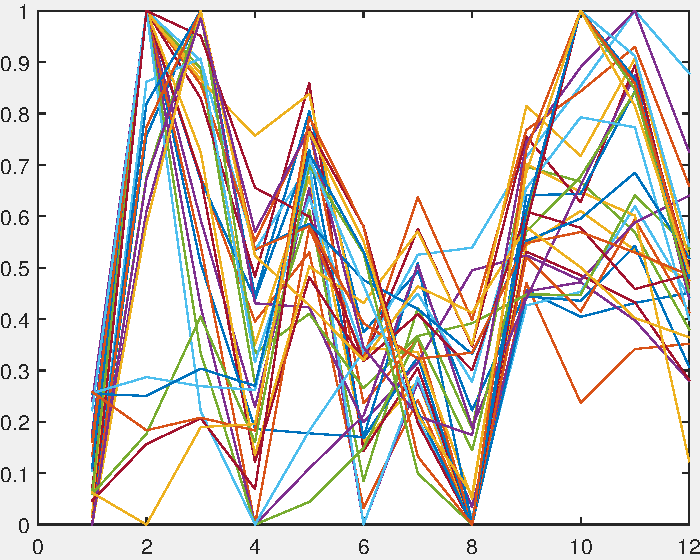
\includegraphics[width=\textwidth]{image/Ch5/MFCC.pdf}
                \caption{MFCCs}
        \end{subfigure}%
        ~ 
        \begin{subfigure}[b]{0.5\textwidth}
                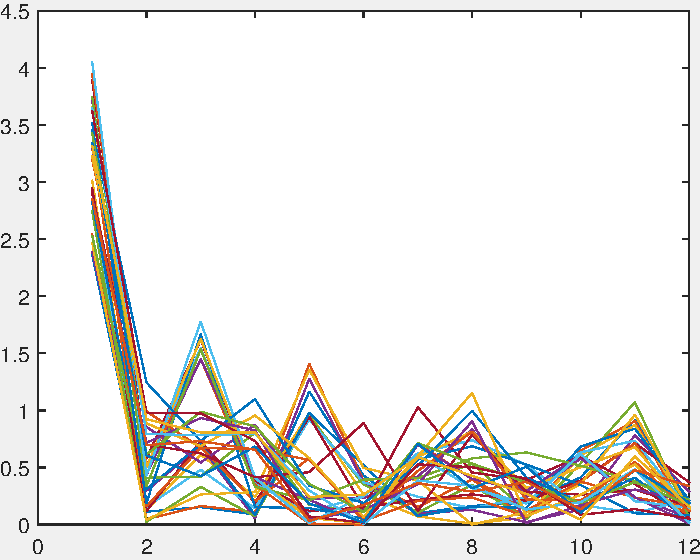
\includegraphics[width=\textwidth]{image/Ch5/MelCC.pdf}
                \caption{MWSCCs}
        \end{subfigure}
        \\
                \begin{subfigure}[b]{0.5\textwidth}
                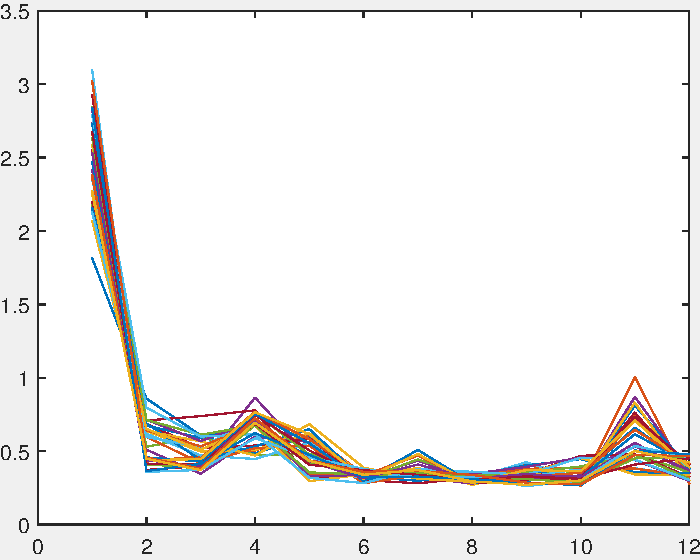
\includegraphics[width=\textwidth]{image/Ch5/avgPWSCC.pdf}
                \caption{Averaged AWSCCs}
        \end{subfigure}%
        ~ 
        \begin{subfigure}[b]{0.5\textwidth}
                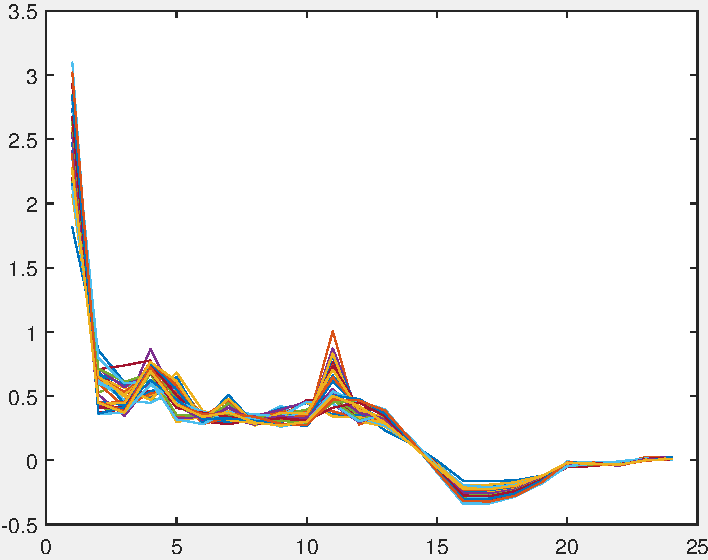
\includegraphics[width=\textwidth]{image/Ch5/deltaPWSCC.pdf}
                \caption{Delta-AWSCCs}
        \end{subfigure}
        \caption[The feature vectors for 31 syllables of the single species, \textit{Assa darlingtoni}]{The feature vectors for 31 syllables of the single species, \textit{Assa darlingtoni}. The x-axis is the feature index and y-axis
is the feature value. Note that the feature vectors for averaged AWSCCs (c) and delta-AWSCCs (d) are more highly correlated than for the other two methods (a) and (b).}       
        \label{fig:Ch5_feature}
\end{figure}


As for SFs and MFCCs, the averaged classification accuracy is much lower than AWSCCs, which is 83.2\% and 91.8\%, respectively. To explore the reason for the improvement of the proposed feature, the frog call classification accuracy of all frog species is shown in Table \ref{tab:featureComp}. However, only the features that use the SVM classifier are shown, because averaged accuracy of the k-NN classifier (93.2\%) is lower than the SVM classifier (94.64\%). 


\begin{table}[htb!]
\centering
\caption[Classification accuracy of five features for the classification of twenty-four frog species using the SVM classifier]{Classification accuracy of five features for the classification of twenty-four frog species using the SVM classifier. Here, Avg AWSCCs means the averaged AWSCCs.}
\label{tab:featureComp}
\resizebox{0.8\textwidth}{!}{
\begin{tabular}{llllll}
\hline\hline
\multirow{2}{*}{{\bf Code}} & \multicolumn{5}{c}{{\bf Classification accuracy (\%)}}                         \\ \cline{2-6} 
                            & {\bf SFs} & {\bf MFCCs} & {\bf MelCCs} & {\bf Avg AWSCCs} & {\bf Delta-AWSCCs} \\ \hline
ADI                         & 76.7  $\pm$   15.3 & 80.0  $\pm$   22.1   & 83.3  $\pm$   16.7    & 100.0  $\pm$   0.0        & 100.0  $\pm$   0.0          \\ 
CPA                         & 86.7  $\pm$   16.3 & 100.0  $\pm$   0.0   & 93.3  $\pm$   13.3    & 100.0  $\pm$   0.0        & 100.0  $\pm$   0.0          \\ 
LCA                         & 93.3  $\pm$   15.3 & 100.0  $\pm$   0.0   & 100.0  $\pm$   0.0    & 100.0  $\pm$   0.0        & 100.0  $\pm$   0.0          \\ 
LCS                         & 70.0  $\pm$   23.3 & 63.3  $\pm$   27.7   & 96.7  $\pm$   10.0    & 93.3  $\pm$   13.3        & 96.7  $\pm$   10.0          \\ 
LFX                         & 91.7  $\pm$   8.3  & 93.3  $\pm$   8.2    & 93.3  $\pm$   8.2     & 100.0  $\pm$   0.0        & 100.0  $\pm$   0.0          \\ 
LGA                         & 30.0  $\pm$   45.8 & 100.0  $\pm$   0.0   & 100.0  $\pm$   0.0    & 100.0  $\pm$   0.0        & 100.0  $\pm$   0.0          \\ 
LLA                         & 92.7  $\pm$   8.1  & 98.7  $\pm$   2.7    & 98.0  $\pm$   4.3     & 100.0  $\pm$   0.0        & 100.0  $\pm$   0.0          \\ 
LNA                         & 78.6  $\pm$   14.6 & 94.3  $\pm$   9.5    & 95.7  $\pm$   9.1     & 100.0  $\pm$   0.0        & 100.0  $\pm$   0.0          \\ 
LRA                         & 40.0  $\pm$   30.0 & 10.0  $\pm$   20.0   & 100.0  $\pm$   0.0    & 90.0  $\pm$   20.0        & 98.2  $\pm$   6.5          \\ 
LUA                         & 60.0  $\pm$   20.0 & 100.0  $\pm$   0.0   & 86.7  $\pm$   22.1    & 100.0  $\pm$   0.0        & 100.0  $\pm$   0.0          \\ 
LVV                         & 100.0  $\pm$   0.0 & 96.7  $\pm$   10.0   & 80.0  $\pm$   22.1    & 93.3  $\pm$   13.3        & 100.0  $\pm$   0.0          \\ 
MFS                         & 90.0  $\pm$   15.3 & 76.7  $\pm$   21.3   & 90.0  $\pm$   15.3    & 100.0  $\pm$   0.0        & 100.0  $\pm$   0.0          \\ 
MFI                         & 90.0  $\pm$   30.0 & 100.0  $\pm$   0.0   & 100.0  $\pm$   0.0    & 100.0  $\pm$   0.0        & 100.0  $\pm$   0.0          \\ 
PKN                         & 90.0  $\pm$   20.0 & 100.0  $\pm$   0.0   & 100.0  $\pm$   0.0    & 100.0  $\pm$   0.0        & 100.0  $\pm$   0.0          \\ 
PCA                         & 72.5  $\pm$   20.8 & 77.5  $\pm$   20.8   & 95.0  $\pm$   10.0    & 92.5  $\pm$   11.5        & 100.0  $\pm$   0.0          \\ 
PRI                         & 45.0  $\pm$   35.0 & 80.0  $\pm$   33.2   & 100.0  $\pm$   0.0    & 100.0  $\pm$   0.0        & 100.0  $\pm$   0.0          \\ 
RSS                         & 50.0  $\pm$   50.0 & 100.0  $\pm$   0.0   & 100.0  $\pm$   0.0    & 100.0  $\pm$   0.0        & 100.0  $\pm$   0.0          \\ 
ULA                         & 93.3  $\pm$   13.3 & 100.0  $\pm$   0.0   & 100.0  $\pm$   0.0    & 100.0  $\pm$   0.0        & 100.0  $\pm$   0.0          \\ \hline\hline
\end{tabular}
}
\end{table}

Table \ref{tab:featureComp} lists the classification accuracy of all 18 frog species with five features. It can be seen from the table that delta-AWSCCs have an accuracy greater than 95\% for all frog species. Compared with averaged AWSCCs, the classification accuracy of \textit{Pseudophryne coriacea} (PCA) and \textit{Litoria verreauxii verreauxii} (LVV) are improved to 100\%; it might be that the delta-AWSCCs include the dynamic information of frog calls. For  \textit{Litoria revelata} (LRA), both the classification accuracy of averaged AWSCCs and delta-AWSCCs are lower than 100\%; this is because the dominant frequency is quite similar with multiple frog species including \textit{Assa darlingtoni} (ADI), \textit{Litoria nasuta} (LNA) and \textit{Litoria verreauxii verreauxii} (LVV). However, the classification of \textit{Litoria revelata} (LRA) is 100\% using Mel-scale based techniques, because the Mel-scale has a better frequency resolution for \textit{Litoria chloris} (LCS) within its dominant frequency range. In Table \ref{tab:manySpecies}, the classification accuracy of SFs and MFCCs is lower than the other three features, at only 84.2\% and 92.8\%, respectively. 


The statistical significance of the results is shown in Table \ref{tab:t-test}. The classification accuracy of average AWSCCs is not significantly lower than the delta-AWSCCs. However, the classification accuracy of MWSCCs, MFCCs and SFs is significantly lower than delta-AWSCCs. 

\begin{table}[htb!]
\caption[Paired statistical analysis of the results in Table~\ref{tab:featureComp}]{Paired statistical analysis of the results in Table~\ref{tab:featureComp}. For the classification accuracy of each frog species, the paired Student t-test was conducted \citep{tanton2005encyclopedia}.}
%McNemar's test \citep{mcnemar1947note} was adopted for comparing the classification results based on the binary results of 340 syllables (0 = incorrect classified, 1 = corrected classified)

\centering
\label{tab:t-test}
\resizebox{0.85\textwidth}{!}{
\begin{tabular}{lll}
\hline\hline
{\bf Pairs}                  & \multicolumn{2}{l}{{\bf t-test results}}                               \\ \hline
%\multicolumn{3}{l}{{\bf Student t-test on test results based on species}}                           \\ 
Delta-AWSCCs - Avg AWSCCs    & \multicolumn{2}{l}{t=1.95 (not significant)}                         \\ 
Delta-AWSCCs - MWSCCs        & \multicolumn{2}{l}{t=3.41 (significant at p \textless 0.01, df =17)} \\ 
Delta-AWSCCs - MFCCs         & \multicolumn{2}{l}{t=2.91 (significant at p \textless 0.01, df =17)} \\ 
Delta-AWSCCs - SFs           & \multicolumn{2}{l}{t=5.52 (significant at p \textless 0.001, df =17)} \\ \hline\hline
%\multicolumn{3}{l}{{\bf McNemar's test on test results based on syllales}}                          \\ \hline
%Delta AWSCCs - Avg AWSCCs    & \multicolumn{2}{l}{p=0.3613, not significant}                        \\ \hline
%Delta AWSCCs - MWSCCs        & \multicolumn{2}{l}{p=0.3601, not significant}                            \\ \hline
%Delta AWSCCs - MFCCs         & \multicolumn{2}{l}{p=0.0375, significant}                            \\ \hline
%Delta AWSCCs - SFs           & \multicolumn{2}{l}{p=0.0001, highly significant}                            \\ \hline
\end{tabular}
}
\end{table}


Since our wavelet packet tree for feature extraction is obtained based on the frog species to be classified, two more experiments are used for further evaluation. The first experiment is to classify first ten frog species (No.1-10); the second is to classify the first fourteen frog species (No.1-14) (see Table \ref{tab:parameter}). The wavelet packet tree for classifying ten and fourteen frog species is shown in Figure~\ref{fig:wpTree}, which is different from the tree for classifying eighteen frog species. However, the Mel-scaled wavelet packet tree is the same for all experiments (see Figure~\ref{fig:melTree}). The classification results are shown in Table \ref{tab:manySpecies}. Since the classification accuracy with averaged AWSCCs is very high for classifying ten and fourteen frog species, the delta-AWSCCs is not included in this experiment. Table \ref{tab:manySpecies} shows that averaged AWSCCs can achieve the highest classification accuracy for classifying different numbers of frog species. Since the averaged AWSCCs is adaptively extracted based on the data, more frog species do not cause a large decrease in the classification accuracy.  



\begin{figure}[htb!] % Example image
\center{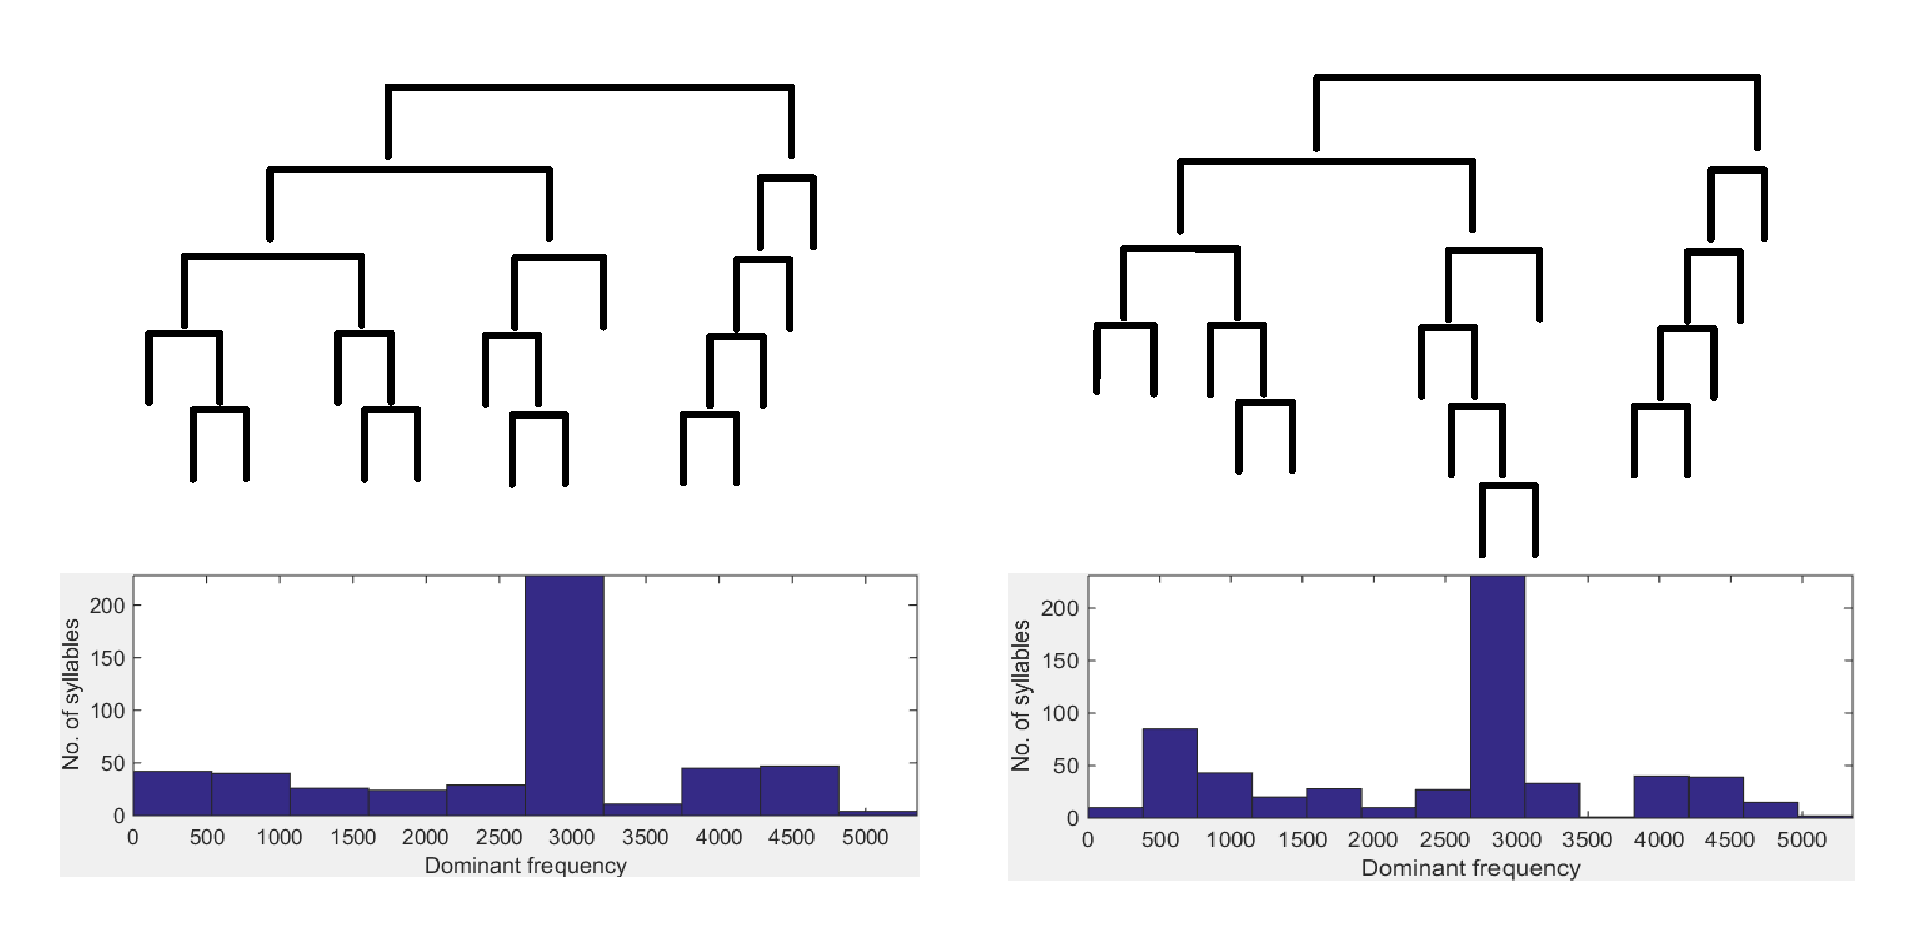
\includegraphics[width=0.95\linewidth, height= 0.5\linewidth]{image/Ch5/tree15vs10.pdf}}
\caption{Wavelet packet tree based on adaptive frequency scale for classifying ten and fifteen frog species.}
\label{fig:wpTree} 
\end{figure}


\begin{figure}[htb!] % Example image
\center{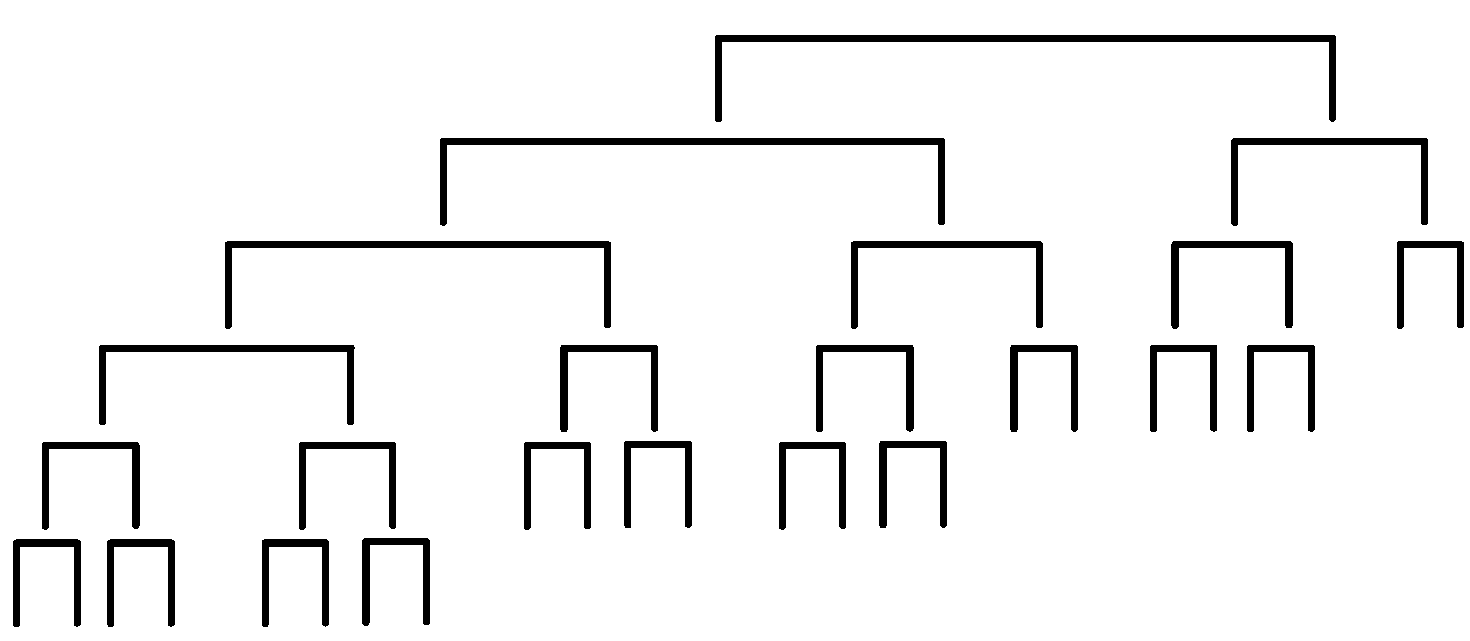
\includegraphics[width=0.8\linewidth, height= 0.4\linewidth]{image/Ch5/MelTree.pdf}}
\caption{Mel-scaled wavelet packet tree for frog call classification.}
\label{fig:melTree} 
\end{figure}


\begin{table}[htb!]
\centering
\caption{Classification accuracy (\%) for classifying different number of frog species with four feature sets.}
\label{tab:manySpecies}
\resizebox{0.85\textwidth}{!}{
\begin{tabular}{lllll}
\hline\hline
{\bf Features} & {\bf SFs} & {\bf MFCCs} & {\bf MWSCCs} & {\bf Averaged AWSCCs} \\ \hline
18 frog species  & 84.2 $\pm$ 10.5 & 92.8 $\pm$ 11.0  &             97.6 $\pm$ 5.7 &  99.0 $\pm$ 4.6                     \\ 
14 frog species  & 89.6 $\pm$ 9.7  & 94.4 $\pm$ 8.5   &             99.2 $\pm$ 2.6 &     100.0 $\pm$ 0.0                 \\ 
10 frog species  & 94.6 $\pm$ 8.7   &  95.8 $\pm$ 8.6     &             100.0 $\pm$ 0.0 &   100.0 $\pm$ 0.0                   \\ \hline\hline
\end{tabular}
}
\end{table}


\subsection{Comparison under different SNRs}
To further evaluate the robustness of the proposed feature, a Gaussian noise signal, with SNR of 40 dB, 30 dB, 20 dB, and 10 dB, is added to the original signal. The noise is added after syllable segmentation, because this chapter focuses on the development of novel features for classification rather than the segmentation method. The classification accuracy with five features under different SNRs is shown in Figure~\ref{fig:snr}. Compared with MFCCs and MWSCCs, SFs has a stronger anti-noise performance, because the dominant frequency of SFs has a small variation under low SNR. Correspondingly, the adaptive frequency scale also has a small variation, because it is generated by means of applying the k-means clustering algorithm to the dominant frequency. Therefore, our proposed feature has a stronger anti-noise performance than other cepstral features (MFCCs and MWSCCs). 

\begin{figure}[htb!] % Example image
\center{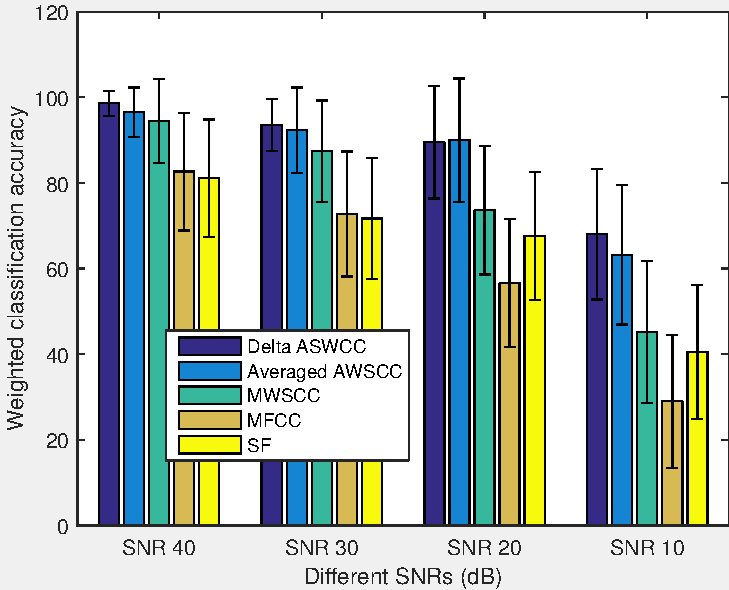
\includegraphics[width=0.6\linewidth, height = 0.4\linewidth]{image/Ch5/snr.pdf}}
\caption{Sensitivity of five features for
different levels of noise contamination.}
\label{fig:snr} 
\end{figure}

\subsection{Feature evaluation using the real world recordings}
Table \ref{tab:realField} shows the classification accuracy comparison using our proposed feature to classify eight frog species obtained from the JCU recordings. Since calls of some frog species in the JCU recordings do not have oscillation structure, SFs are not included for the comparison. Compared with other referred features, our proposed feature also achieves the best classification performance.
Since the JCU recordings often have multiple calls from different frog species, spectral peak track occasionally can not capture the specific frog species (labelled species for that syllable), but other frog species to be classified; however, applying k-mean clustering to the dominant frequency calculated from the spectral peak track can reduce this deviation. Therefore, the frequency scale used for the WPD can be accurately achieved, which still leads to a high classification accuracy with the proposed feature.

% Please add the following required packages to your document preamble:
% \usepackage{multirow}
\begin{table}[htb!]
\centering
\caption{Classification accuracy using the JCU recordings.}
\label{tab:realField}
\resizebox{0.6\textwidth}{!}{
\begin{tabular}{lll}
\hline\hline
\multirow{2}{*}{\textbf{Feature set}} & \multicolumn{2}{l}{\textbf{Classification accuracy (\%)}} \\ \cline{2-3} 
                                   & \textbf{k-NN}             & \textbf{SVM}             \\ \hline
MFCCs                              &       67.5 $\pm$ 13.2                    &    70.8 $\pm$ 14.1                     \\ 
MWSCCs                             &       90.4  $\pm$ 9.2                   &   91.6 $\pm$ 8.7                    \\ 
Averaged AWSCCs                    &    94.1  $\pm$  6.3 &                         94.5 $\pm$ 5.8  \\ 
Delta-AWSCCs                       &         97.0   $\pm$ 5.2                &   \textbf{97.4  $\pm$  5.4 }                     \\ \hline\hline
\end{tabular}
}
\end{table}


\section{Summary and limitations}
In this chapter, a novel feature extraction method for frog call classification is developed using the adaptive frequency scaled wavelet packet decomposition. With segmented syllables, spectral peak track is first extracted from each syllable. Then, track duration, dominant frequency, and oscillation rate are calculated based on each track. Next, a k-means clustering algorithm is applied to the dominant frequency, which generates the frequency scale for WPD. Finally, a new feature set, AWSCCs, is calculated. Since the feature extraction method is developed based on the data itself, the wavelet packet tree varies according to the frog species to be classified. Compared with the Mel-scaled WPD tree, the proposed adaptive wavelet packet tree can better fit the dominant frequency distribution of the frog species to be classified. With the proposed frequency scale, the call characteristics of those frog species to be classified can be enhanced, while the background noise and calls from other animals will be suppressed. Therefore, the proposed feature sets can achieve a higher accuracy for the classification of frog calls than others. Meanwhile, since the frequency scale is calculated based on the dominant frequency of those frog species to be classified, our proposed wavelet tree structure is more accurate and efficient in classifying the frog calls when compared with Mel-scale (Figure~\ref{fig:wpTree} and Figure~\ref{fig:melTree}).


The feature extraction algorithm is designed for classifying frog calls. For frog calls, the typical structure in a spectrogram is frequency contour (named spectral peak track in this chapter) which is within a given frequency range starting at a given time \citep{mellinger2011method}. For other organisms that have similar frequency contour structures such as the whistles of dolphins, and chirps of birds \citep{chen2006semi}, spectral peak tracks can also be extracted from the spectrograms of their calls. Based on those spectral peak tracks, dominant frequency can be calculated. For the subsequent analysis, the features can be calculated using the same process as described in this chapter. For those organisms without clear frequency contour structure, this proposed method can also be used by enhancing the frequency contour structure, which can be realised by applying a small window size and a large window overlap to the recording waveform. 


The oscillation rate is calculated based on the spectrogram, which is generated by applying STFT to the waveform. However, when the temporal gap is smaller than the window size used for STFT, the oscillation structure will disappear. Therefore, finding new techniques for translating the 1-D signal to 2-D signal is our future direction. Since the frequency scale is generated based on the dominant frequency, this technique can be applied to other organisms that have clear frequency contour structure. Modifying this algorithm to those organisms without a clear frequency contour structure needs to be solved. 
This research also plans to include additional experiments that test a wider variety of audio data from different geographical and environment conditions. Other animal calls such as birds, insects, and whales can also be studied. Furthermore, the idea of developing new features based on the data itself will be explored.


